\chapter{数理统计}
\label{chap:mathematical-statistics}

概率论假定分布已经给定，再计算事件概率和随机变量的平均。本章把方向反过来：我们只
看到有限个带噪读数
\[
  Y_i=\theta+\varepsilon_i,\qquad i=1,\ldots,n,
\]
却希望认识未知的信号、噪声分布，乃至下一次读数。样本平均看似给出了答案，但它立即
留下几项问题。读数是否来自希望推广到的总体？两个不同信号会不会产生相同的观测
分布？异常读数会怎样改变结论？反复选择模型和查看结果后，原有的不确定性说明是否仍然
可信？

\term{数理统计}（mathematical statistics）研究如何由有限观测推断产生观测的规律，
以及如何量化这种推断的不确定性。一个统计结论必须先有目标与观测机制，才有适用的估计方法；
给出估计后，还要在重复抽样或后验分布中说明误差。若按数据选中一个结果，
又需把选择与停止纳入保证。目标从参数转成未来分布时，评价尺度和表示方法随之改变；
模型比较与新增观测则进一步要求明确比较口径和信息预算。
本章沿这些问题组织工具，始终追踪数据包含什么信息，以及当前结论究竟由哪些条件支持。

\section{推断目标与数据来源}
\label{sec:stats-targets-data-sources}

统计推断先要明确要回答哪个总体问题，再说明观测如何产生。相同的数据表，
在不同抽样制度下可能对应不同总体；相同的模型，某个目标也可能无法由观测分布唯一确定。
本节把目标、可识别性、抽样与缺失机制放在一起，为后面的估计与误差声明确定共同前提。

\subsection{统计模型与推断目标}
\label{sec:statistics-model-target}

\subsubsection{模型、统计量与目标泛函}

\begin{definition}[统计模型与统计量]
  \label{def:statistics-model-statistic}
\term{统计模型}（statistical model）是一族候选分布
\[
  \mathcal{P}=\{P_\vartheta:\vartheta\in\Theta\}.
\]
这些分布定义在同一个可测观测空间上，参数\(\vartheta\)是描述候选分布的未知索引。观测
\(\bm{Y}=(Y_1,\ldots,Y_n)\)由其中某个分布产生，但真实索引不可见。参数未必是
一个物理常数；它也可以是一组回归系数、一个混合比例，或者无限维的分布函数。

\term{统计量}（statistic）是只依赖样本的可测函数
\(T(\bm{Y})\)。当统计量被设计来逼近某个未知目标
\(\tau(\vartheta)\)时，它称为\term{估计量}（estimator），通常记为
\(\widehat{\tau}\)。在一批已经观测的数据\(\bm{y}\)上算出的
\(\widehat{\tau}(\bm{y})\)是\term{估计值}（estimate）。参数属于模型，估计量
在重复抽样中是随机变量，估计值则是一次计算得到的数；混淆三者会使“偏差”和
“不确定性”失去对象。
\end{definition}

推断目标可以有不同层次。估计\(\theta\)是在参数空间中找一个点；估计分布函数
\(F(y)\)是在函数空间中恢复整体规律；预测未来观测\(Y_{n+1}\)则还要保留新噪声。
即使都输出一个数，它们回答的也不是同一个问题。例如
\(\overline{Y}\)可估计位置\(\theta\)，而预测下一次读数还需要噪声尺度。
一般地，目标写成映射\(\tau:\Theta\to\mathcal A\)，其中
\(\mathcal A\)可以是标量、向量、函数或概率分布。能够只由可观察分布决定的目标也可
进一步写成分布泛函。估计误差还必须配合损失
\(\ell:\mathcal A\times\mathcal A\to[0,\infty]\)解释；向量目标的坐标平方误差、
总平方误差和某个方向上的误差是不同口径，不能只写“估计准确”。

在有限方差位置模型\(Y_i=\theta+\varepsilon_i\)中，若误差独立、均值为零且方差为
\(\sigma^2\)，则
\[
  \mathbb{E}_\theta[\overline Y]
  =\theta+\frac1n\sum_{i=1}^n\mathbb{E}[\varepsilon_i]
  =\theta,\qquad
  \operatorname{Var}_\theta(\overline Y)
  =\frac1{n^2}\sum_{i=1}^n\operatorname{Var}(\varepsilon_i)
  =\frac{\sigma^2}{n}.
\]
无偏性来自零均值，\(1/n\)方差缩减还使用了独立性；若误差相关，方差中必须保留
协方差项。

\subsubsection{识别、等价模型与推断边界}

数据充足之前还要问目标能否由观测区分。
\begin{definition}[目标可识别性]
  \label{def:statistics-identifiability}
  给定统计模型\(\{P_\vartheta:\vartheta\in\Theta\}\)和目标泛函\(\tau:\Theta\to\mathcal T\)，若对所有\(\vartheta_1,\vartheta_2\in\Theta\)有
\[
  P_{\vartheta_1}=P_{\vartheta_2}
  \quad\Longrightarrow\quad
  \tau(\vartheta_1)=\tau(\vartheta_2),
\]
就称目标\(\tau\)在模型中是\term{可识别的}（identifiable）。
\end{definition}
取
\(\tau(\vartheta)=\vartheta\)时，这一定义才退化为参数可识别。可识别性是总体分布
层面的性质，不是有限样本算法的表现。

\begin{example}[混合成分的标签交换]
\label{ex:statistics-mixture-label-switching}
设观测来自二成分高斯混合
\[
  p(y)=\pi\phi(y;\mu_1,\sigma^2)
       +(1-\pi)\phi(y;\mu_2,\sigma^2).
\]
把\((\pi,\mu_1,\mu_2)\)换成
\((1-\pi,\mu_2,\mu_1)\)不改变分布。若“第一成分”只表示编号，参数便有两种等价
表示；添加\(\mu_1<\mu_2\)之类约束可以固定表示，却没有创造新的观测信息。
\end{example}

另一种失败来自来源一起出错。若所有温度计都有未知共同偏移\(b\)，模型为
\(Y_i=\theta+b+\varepsilon_i\)，观测只识别\(\theta+b\)，不能分别识别
\(\theta\)和\(b\)。增加同型号温度计会减小随机噪声，却不会消除共同偏差。由此可见，
“有很多数据”“目标可识别”和“目标容易准确估计”是三项不同判断。

不可识别还直接限制任何估计程序。若
\(P_{\vartheta_1}=P_{\vartheta_2}\)但
\(\tau(\vartheta_1)\neq\tau(\vartheta_2)\)，取两目标值距离的三分之一为
\(\epsilon>0\)。任何只依赖样本的估计量\(\widehat\tau_n\)在两种机制下具有相同
分布，因而不可能同时满足
\[
  \mathbb{P}_{\vartheta_j}
  \left\{\lVert\widehat\tau_n-\tau(\vartheta_j)\rVert<\epsilon\right\}
  \longrightarrow1,\qquad j=1,2.
\]
因为两个半径为\(\epsilon\)的球不相交，同一个估计量分布不可能把趋近于一的概率
同时赋给它们。这证明了：不可识别目标不能靠增加同类样本在全部等价机制下一致恢复。

\subsection{抽样制度与目标总体}
\label{sec:statistics-sampling-population}

\subsubsection{总体、抽样与权重}

统计结论必须先回答“想对谁成立”。\term{目标总体}（target population）是推断希望
覆盖的对象、时间和条件的集合；\term{抽样制度}（sampling regime）描述观测如何从
这些对象产生。若样本只来自工作日的一个传感器，模型本身不能把结论自动推广到周末或
另一批设备。

独立同分布抽样把每个\(Y_i\)视为来自同一分布的独立重复。配对抽样则把
\((Y_{i,A},Y_{i,B})\)视为一个单位，例如同一对象在两种条件下的读数。此时差值
\(D_i=Y_{i,A}-Y_{i,B}\)才是独立单位；把两列拆成\(2n\)个独立记录会丢失配对信息。
分层抽样预先按群组分别抽取，成组抽样则一次抽取整个设备、班级或用户群。两者的
独立单位和加权方式不同。

\subsubsection{条件分母、相关性与信息量}

配对的收益取决于对内协方差：
\[
  \operatorname{Var}(D_i)
  =\operatorname{Var}(Y_{i,A})+\operatorname{Var}(Y_{i,B})
   -2\operatorname{Cov}(Y_{i,A},Y_{i,B}).
\]
正协方差会降低差值方差，负协方差则可能使配对更差；“同一对象测两次”本身并不保证
精度提高。

设目标总体中群组\(g\)的比例为\(\pi_g\)，群组均值为\(\mu_g\)，则总体均值为
\[
  \mu=\sum_g\pi_g\mu_g.
\]
总体指标可能很好，却掩盖某个小群组的严重误差。若群组中有\(n_g\)个独立Bernoulli
结果，样本比率\(\widehat p_g\)的方差为
\[
  \operatorname{Var}(\widehat p_g)
  =\frac{p_g(1-p_g)}{n_g}.
\]
这里把\(n_g\)视为固定正整数。若群组样本数
\(N_g=\sum_i\mathbb{I}\{G_i=g\}\)也是随机的，则
\(\widehat p_g\)只在\(N_g>0\)时有定义，且上述方差是给定\(N_g\)后的条件方差；
无条件误差还要平均随机分母，并处理\(N_g=0\)事件。不确定性由实际相关分母决定，
而不是总样本量\(n\)。报告群组公平性或来源质量时，应同时报告分母、抽样方式和区间，
不能只排列百分比。

已知入样概率时，权重可以把抽样分布重新接回目标总体。令\(S\in\{0,1\}\)表示一个
总体对象是否入样，\(\rho(Z)=\mathbb{P}(S=1\mid Z)\)，并假设
\(S\mathrel{\perp}Y\mid Z\)、\(\rho(Z)>0\)以及
\(\mathbb{E}[|Y|/\rho(Z)]<\infty\)。条件期望给出
\[
  \mathbb{E}\left[\frac{SY}{\rho(Z)}\right]
  =\mathbb{E}\left[
    \frac{\mathbb{E}[S\mid Y,Z]Y}{\rho(Z)}
  \right]
  =\mathbb{E}[Y].
\]
这条逆概率恒等式恢复的是明确的总体平均。若某一区域\(\rho(Z)=0\)，或者入样在给定
\(Z\)后仍依赖未观测的\(Y\)，等式便不能由现有数据推出。

记录数也不等于独立信息量。若同一来源复制一条记录十次，样本平均的显示分母增大，
实际信息却没有增加。时间序列中的相邻读数可能共享漂移；群组内记录可能共享设备偏差。
这类依赖应通过按群组建模、块抽样或
第~\ref{chap:stochastic-processes-and-approximation}章的相关过程工具处理，而不能
继续套用独立样本方差。

时间抽样还会改变目标本身。若传感器每分钟记录一次，而目标是“一天中随机时刻的平均
读数”，等间隔采样与目标一致；若只在告警后加密采样，朴素平均就会过度代表异常时段。
一种修正方式是记录每个时段被抽中的概率并作逆概率加权，但这要求所有目标时段都有正的
入样概率。完全未覆盖的夜间时段不能靠增大已有权重恢复。抽样日志因此也是统计数据的一
部分。

抽样制度与分析单位应在看结果前确定。假设十台设备各产生一千条记录，而处理实际随机
分配给设备，那么有效随机化单位是十台设备，不是一万条记录。记录内噪声可以帮助估计
每台设备的均值，却不能把处理效应的独立单位扩充到一万。这个区别会同时影响标准误、
置换方式和训练测试划分。

\subsubsection{缺失、选择与可忽略性}
\label{sec:statistics-missingness-observation}

不完整观测带来另一类问题。令\(R=1\)表示\(Y\)被观察到，\(X\)为始终可见变量。
\term{完全随机缺失}（missing completely at random, MCAR）要求
\[
  R\mathrel{\perp}(X,Y).
\]
\term{随机缺失}（missing at random, MAR）要求
\[
  R\mathrel{\perp}Y\mid X,
\]
即给定已观测协变量后，缺失概率不再依赖缺失值本身。
\term{非随机缺失}（missing not at random, MNAR）则允许这种剩余依赖。

多个变量可能按不同模式缺失，此时“已观测变量”随模式改变，不能用一个固定条件集概括全部MAR要求。
\begin{definition}[观测模式与缺失机制]
  \label{def:statistics-missingness}
  设完整数据为\(\bm Z=(Z_1,\ldots,Z_d)\)，观测指示\(\bm R\in\{0,1\}^d\)。对每种模式\(\bm r\)，定义
  \[
    O(\bm r)=\{j:r_j=1\},\qquad M(\bm r)=\{j:r_j=0\}.
  \]
  实际记录为\((\bm r,\bm Z_{O(\bm r)})\)。令\(g(\bm r\mid\bm z)\)为给定完整数据时的模式概率核。若对每种\(\bm r\)都存在只依赖已见坐标的可测函数\(g_{\bm r}\)，使
  \[
    g(\bm r\mid\bm z)=g_{\bm r}(\bm z_{O(\bm r)})
  \]
  对完整数据分布几乎处处成立，则称机制为MAR。若\(g(\bm r\mid\bm z)\)对全部模式均不依赖\(\bm z\)，则为MCAR；若MAR条件失败，则为MNAR。
\end{definition}
例如在二维数据中，模式\((1,0)\)的出现概率可依赖\(Z_1\)，却不能依赖未见的\(Z_2\)；模式\((0,1)\)反过来可以依赖\(Z_2\)，却不能依赖\(Z_1\)。这是对每种模式分别施加的条件，不能只在当前观测到的某一模式上核对。“随机缺失”也不等于“缺失标记完全随机”，后者对应更强的MCAR。

当\(\mathbb{P}(R=1)>0\)时，MCAR下完整案例仍代表总体，但效率降低。MAR下可建模
\(\mathbb{P}(R=1\mid X)\)并加权，或建模\(Y\mid X\)后插补；两者都依赖模型和
正值条件。MNAR通常不能只靠已观测数据识别，需要机制假设、外部信息或敏感性分析。
所谓“缺失机制可忽略”还要求推断参数与缺失机制参数可分离；Bayes分析中还涉及先验
可分离。数据表中的一个缺失标记本身不能证明属于哪种机制。

识别障碍在有界结果上已经出现。若\(0\leq Y\leq1\)且
\(\mathbb{P}(R=0)>0\)，观测数据只给出已见部分的\(RY\)与缺失指示；把所有未见
\(Y\)设为\(0\)或设为\(1\)会产生相同观测，却给出不同总体均值。因此不加机制条件
时只能得到
\[
  \mathbb{E}[RY]
  \leq\mathbb{E}[Y]
  \leq\mathbb{E}[RY]+\mathbb{P}(R=0).
\]
两个端点分别可由把全部未见结果设为\(0\)或\(1\)达到，所以仅凭上述信息不能继续
收紧。若MAR成立，并令
\(\pi(X)=\mathbb{P}(R=1\mid X)>0\)，则第
~\ref{sec:statistics-sampling-population}节的逆概率恒等式在这里化为
\[
  \mathbb{E}\left[\frac{RY}{\pi(X)}\right]
  =\mathbb{E}[Y].
\]
正值条件负责覆盖，条件独立负责把未见结果接回已见结果；权重很大时，即使目标可识别，
有限样本方差仍可能很高。

\section{参数推断与效率}
\label{sec:stats-parameter-inference-efficiency}

目标与观测机制确定后，才有意义讨论如何估计，以及哪种估计误差更小。
似然和估计方程从样本构造点估计，偏差、方差与渐近理论评价其重复抽样表现；
Bayes方法进一步把先验信息与观测合并，层次模型则说明多个群体怎样共享信息。
频率与Bayes结论使用不同的概率对象，评价时应保留这个区别。

\subsection{似然、估计方程与稳健性}
\label{sec:statistics-likelihood-robustness}

\subsubsection{似然与充分统计量}

给定观测\(\bm{y}\)后，\term{似然}（likelihood）
\[
  L(\vartheta;\bm{y})=p_\vartheta(\bm{y})
\]
相对于模型共同的参考测度定义，把数据固定，把参数看作待比较的变量。似然不是参数的
概率分布；只有再指定先验并归一化后，才得到后验分布。最大似然估计选择
\(\widehat\vartheta_{\mathrm{MLE}}\in\argmax_\vartheta L(\vartheta;\bm{y})\)，
通常等价于最小化负对数似然\scite{vanderVaart1998asymptotic}

对\(Y_i\overset{\mathrm{iid}}{\sim}\mathcal{N}(\theta,\sigma^2)\)，且
\(\sigma^2\)已知，
\[
  -\log L(\theta;\bm{y})
  =\frac{1}{2\sigma^2}\sum_{i=1}^n(y_i-\theta)^2+C.
\]
对\(\theta\)求导并令其为零，得到
\(\widehat\theta=\overline y\)。同一个样本平均也可由矩估计得到：总体矩
\(\mathbb{E}_\theta[Y]=\theta\)，于是令样本矩\(\overline Y\)等于总体矩。
似然法依赖完整分布形式，矩估计只使用选定矩条件。

“令导数为零”只寻找内点候选，不保证最大值存在或唯一。例如独立Bernoulli观测的
似然为
\[
  L(p;\bm y)=p^{\sum_i y_i}(1-p)^{n-\sum_i y_i},\qquad p\in[0,1].
\]
当样本同时含有\(0\)和\(1\)时，唯一最大值是样本比例；全为\(1\)或全为\(0\)时，
最大值分别落在边界\(p=1\)或\(p=0\)。若错误地把参数域写成开区间\((0,1)\)，
边界数据甚至只有上确界而没有最大似然估计。

压缩数据会丢掉细节，但有时这些细节与目标参数无关。例如Bernoulli样本的排列不同，只要成功次数相同，似然关于\(p\)的依赖就相同。充分性要求这种“保留全部参数信息”在整个指定模型中成立。
\begin{definition}[充分统计量]
  \label{def:statistics-sufficient-statistic}
  设样本\(\bm Y\)与统计量\(T(\bm Y)\)取值于标准Borel空间。若存在概率核\(K(t,\cdot)\)，对每个\(\vartheta\in\Theta\)都是\(\bm Y\)给定\(T=t\)的正则条件分布版本，而且\(K\)不依赖\(\vartheta\)，则称\(T\)为该模型的\term{充分统计量}（sufficient statistic）。各条件分布的等式按相应\(P_\vartheta^T\)-几乎处处意义理解。
\end{definition}
它是在给定摘要后，样本其余部分不再携带关于参数的信息。在受同一个\(\sigma\)有限测度支配的模型中，若密度可分解为
\[
  p_\vartheta(\bm y)=g_\vartheta(T(\bm y))h(\bm y),
\]
则因子分解定理说明\(T\)对\(\vartheta\)充分。直观地说，给定
\(T(\bm Y)=t\)后，条件密度中的参数因子在归一化时抵消，剩余分布不含
\(\vartheta\)。在有限离散样本空间上，逆向关系也可直接算出。若
\(\bm Y\mid T=t\)的条件质量\(k(\bm y\mid t)\)不依赖参数，则
\[
  p_\vartheta(\bm y)
  =p_\vartheta^T(T(\bm y))k(\bm y\mid T(\bm y)),
\]
也得到所需分解。一般连续情形的条件分布可能集中在低维纤维上，不能把这个离散乘法式未经参考测度核对就当成普通密度恒等式；因子分解定理负责一般受支配模型中的等价性。高斯位置模型中，已知方差时
\(\sum_iY_i\)充分。充分性是相对于指定模型而言的；模型失配后，压缩掉的部分可能正好
暴露失配。

\subsubsection{M估计、矩估计与伪真目标}

似然以指定模型的对数密度作为拟合准则。若目标是中位数、希望减轻异常值影响，或不愿假定完整分布形状，就需要按目标另选样本准则。下面的表达把这些估计方法放在同一个框架中，但不同准则的总体最小点未必相同。
\begin{definition}[M估计]
  \label{def:statistics-m-estimator}
给定可测准则\(\rho(y,\vartheta)\)，当下面的最小点集合非空且存在可测选择时，\term{\(M\)估计}（M-estimation）是从中选出的一个可测统计量：
\[
  \widehat\vartheta
  \in\argmin_{\vartheta\in\Theta}
  \frac1n\sum_{i=1}^n\rho(Y_i,\vartheta).
\]
\end{definition}
可微时，一阶条件是估计方程
\[
  \frac1n\sum_{i=1}^n\psi(Y_i,\widehat\vartheta)=0,
  \qquad
  \psi(y,\vartheta)=\nabla_\vartheta\rho(y,\vartheta).
\]
平方损失给出\(\psi(y,\theta)=\theta-y\)，每个残差的作用随绝对值线性增长。
绝对损失\(\rho(y,\theta)=|y-\theta|\)的总体最小点则是中位数：目标函数的左右
方向导数分别由\(\mathbb{P}(Y<\theta)\)与\(\mathbb{P}(Y>\theta)\)决定，最优条件是
\(\mathbb{P}(Y\leq\theta)\geq1/2\)且
\(\mathbb{P}(Y\geq\theta)\geq1/2\)。因此平方与绝对准则即使使用同一批位置数据，
也在估计不同的总体泛函。

\(M\)估计的一致性需要把经验准则与总体准则连接起来。记
\[
  Q_n(\vartheta)=\frac1n\sum_{i=1}^n\rho(Y_i,\vartheta),
  \qquad
  Q(\vartheta)=\mathbb{E}[\rho(Y,\vartheta)].
\]
假设\(\Theta\)紧，\(Q\)在唯一点\(\vartheta^\star\)取得最小值，并且该最小值
分离，即对每个\(\epsilon>0\)，
\[
  \inf_{\lVert\vartheta-\vartheta^\star\rVert\geq\epsilon}
  Q(\vartheta)>Q(\vartheta^\star).
\]
若\(\sup_{\vartheta\in\Theta}|Q_n(\vartheta)-Q(\vartheta)|
\xrightarrow{\mathbb{P}}0\)，且近似优化误差
\[
  Q_n(\widehat\vartheta_n)-\inf_{\vartheta\in\Theta}Q_n(\vartheta)
  =o_{\mathbb{P}}(1),
\]
其中\(o_{\mathbb{P}}(1)\)表示该随机误差依概率趋于零，则
\(\widehat\vartheta_n\xrightarrow{\mathbb{P}}\vartheta^\star\)。证明只需比较准则：
在任意固定的\(\epsilon\)球外，总体准则有正间隔；当一致偏差和优化误差都小于该
间隔的适当分数时，经验近似最小点不可能位于球外。若参数空间不紧，则必须另证估计点
不会逃向无穷远；若总体最小点不唯一，结论只能指向最小点集合。

若真实分布\(Q\)不属于\(\mathcal P\)，就不能把拟合参数直接解释为真实机制的参数。其总体对数损失目标是：
\begin{definition}[伪真参数]
  \label{def:statistics-pseudo-true-parameter}
相对于共同参考测度的模型密度\(p_\vartheta\)，假定所比较的\(\mathbb E_Q\log p_\vartheta(Y)\)均有定义，且下列最大点集合非空。集合中的任一点
\[
  \vartheta^\star
  \in\argmax_\vartheta\mathbb{E}_Q[\log p_\vartheta(Y)]
\]
称为该准则的\term{伪真参数}（pseudo-true parameter）。
\end{definition}
在经验准则一致逼近、总体极值唯一且分离等条件下，最大似然估计才趋向该点；多个最大点时须改为集合结论。它是模型族中按对数损失最接近
真实分布的点，不必等于科学问题中的真实量。估计量收敛并不自动证明模型正确。

\subsubsection{稳健损失与影响函数}

为了限制异常残差的作用，可使用阈值\(c>0\)的Huber损失
\[
  \rho_c(r)=
  \begin{cases}
    r^2/2,& |r|\leq c,\\
    c|r|-c^2/2,& |r|>c,
  \end{cases}
  \qquad
  \psi_c(r)=
  \begin{cases}
    r,& |r|\leq c,\\
    c\operatorname{sign}(r),& |r|>c.
  \end{cases}
\]
这里\(\psi_c(r)=\rho_c'(r)\)是损失对残差\(r\)的导数。由于
\(\nabla_\theta\rho_c(y-\theta)=-\psi_c(y-\theta)\)，位置估计的参数梯度方程
整体乘以\(-1\)后，等价地写成
\(\sum_i\psi_c(y_i-\widehat\theta)=0\)。小残差仍按平方损失处理，大残差的贡献被截在
\(\pm c\)。代价是：即使高斯模型完全正确，较小的\(c\)也会舍弃一部分有效幅度信息。

总体准则确定估计目标，却没有说明少量异常观测会把它拉动多少。可以向分布\(P\)加入比例为\(\epsilon\)的单点污染，再考察目标的一阶变化。
\begin{definition}[影响函数]
  \label{def:statistics-influence-function}
  设\(T\)为定义在概率分布上的实值或向量值统计泛函，\(\Delta_z\)为全部质量集中在\(z\)的概率测度。假定充分小的正\(\epsilon\)所对应的污染分布仍在\(T\)的定义域内；若右侧极限存在且有限，定义\term{影响函数}（influence function）为
  \[ \operatorname{IF}(z;T,P)=\lim_{\epsilon\downarrow0}
    \frac{T((1-\epsilon)P+\epsilon\Delta_z)-T(P)}{\epsilon}. \]
\end{definition}
例如对均值泛函，\(\operatorname{IF}(z;T,P)=z-\mathbb E_PY\)：同样少量的污染，位置越远，拉动越大。下面把这项敏感性接到估计方程。设统计泛函
\(T(P)\)由
\[
  \mathbb{E}_P[\psi(Y,T(P))]=0
\]
定义，并令\(P_\epsilon=(1-\epsilon)P+\epsilon\Delta_z\)。记
\(A=\mathbb{E}_P[\partial_\theta\psi(Y,T(P))]\neq0\)。假设估计方程在
\(\epsilon=0\)附近可微，微分可移入期望，且所跟踪的根在局部唯一。对
\(\mathbb{E}_{P_\epsilon}[\psi(Y,T(P_\epsilon))]=0\)在
\(\epsilon=0\)处隐式求导，得到
\[
  0=-\mathbb{E}_P[\psi(Y,T(P))]
    +\psi(z,T(P))+A\,T'(0),
\]
第一项为零，因此
\begin{equation}
  \operatorname{IF}(z;T,P)=T'(0)
  =-A^{-1}\psi(z,T(P)).
  \label{eq:statistics-influence-function}
\end{equation}
平方损失的位置影响随\(z\)无界，Huber得分则有界。多维参数时\(A\)是估计方程的
Jacobian矩阵；经验风险中它常表现为Hessian矩阵近似，但只有可微、局部可逆且估计根稳定时，
这种近似才成立。影响函数只描述污染比例在零附近的一阶敏感性，不是任意污染比例下的
误差上界；在回归中，截断残差也不会自动限制极端输入产生的高杠杆影响。

图~\ref{fig:statistics-huber-loss}区分损失本身与它的导数。大残差的Huber损失仍持续增加，并不是把异常观测删除；被限制的是单个残差进入位置估计方程的得分。把“损失增长较慢”直接说成“整个估计量的影响有界”，还需要式~\eqref{eq:statistics-influence-function}中的局部曲率与输入条件。

\begin{figure*}[htbp]
  \centering
  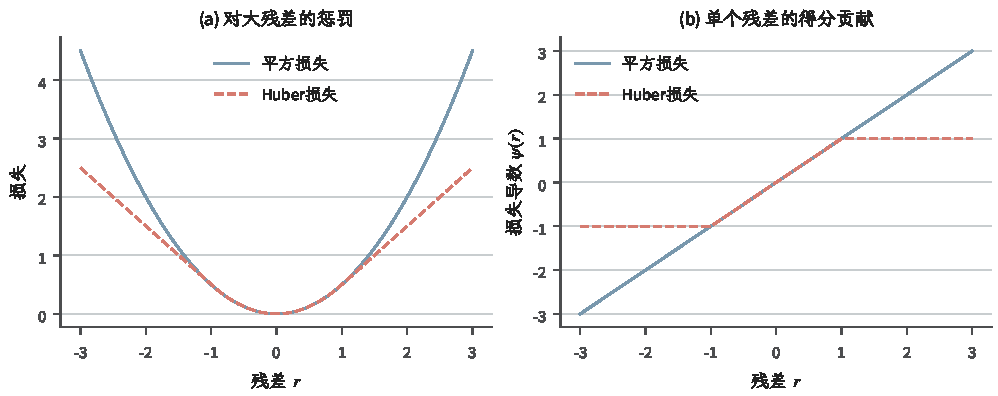
\includegraphics[width=\linewidth]{figures/math-preparation/probability-discrete/statistics-huber-loss.pdf}
  \caption{平方损失与阈值\(c=1\)的Huber损失（解析式教学图）。左图比较惩罚值，右图比较对残差的导数；Huber得分在\([-1,1]\)内截断。横轴是构造残差，不代表实测异常值分布。}
  \label{fig:statistics-huber-loss}
\end{figure*}

\subsection{偏差、方差与估计效率}
\label{sec:statistics-bias-efficiency}

\subsubsection{均方误差与一致性}

估计量的误差既来自系统偏移，也来自样本波动。对标量目标\(\theta\)，
\begin{align}
  \mathbb{E}[(\widehat\theta-\theta)^2]
  &=
  \mathbb{E}[(\widehat\theta-\mathbb{E}\widehat\theta
  +\mathbb{E}\widehat\theta-\theta)^2] \notag\\
  &=
  \operatorname{Var}(\widehat\theta)
  +\bigl(\mathbb{E}[\widehat\theta]-\theta\bigr)^2.
  \label{eq:statistics-mse-decomposition}
\end{align}
交叉项期望为零，因而均方误差等于方差加偏差平方。无偏不等于误差最小；少量偏差可能
换来更大的方差下降。

\begin{definition}[估计量的风险]
  \label{def:statistics-estimator-risk}
给定模型、目标泛函\(\tau\)和非负可测损失\(\ell\)，估计量的\term{风险}（risk）是
\[
  R_\theta(\widehat\tau)
  =\mathbb{E}_\theta[
    \ell(\widehat\tau(\bm Y),\tau(\theta))].
\]
它允许取\(+\infty\)，并随未知参数\(\theta\)变化。
\end{definition}
若\(\bm\theta\in\mathbb{R}^d\)并使用总平方误差，则
\[
  \mathbb{E}\lVert\widehat{\bm\theta}-\bm\theta\rVert_2^2
  =\operatorname{tr}\{\operatorname{Cov}(\widehat{\bm\theta})\}
   +\lVert\mathbb{E}\widehat{\bm\theta}-\bm\theta\rVert_2^2.
\]
这不是每个坐标风险的最大值，也不是任意方向风险。

在高斯位置例子中，取固定中心\(\mu_0\)并令
\(\widetilde\theta=a\overline Y+(1-a)\mu_0\)，则
\[
  \operatorname{MSE}_\theta(\widetilde\theta)
  =\frac{a^2\sigma^2}{n}+(1-a)^2(\mu_0-\theta)^2.
\]
当\(\theta\)接近\(\mu_0\)时，某些\(a<1\)可比无偏的样本均值具有更小有限样本
均方误差；远离中心时，收缩偏差又可能占主导。比较结论必须固定目标、样本量和损失。

当任意\(\epsilon>0\)都满足
\(\mathbb{P}_\theta(|\widehat\theta_n-\theta|>\epsilon)\to0\)时，称估计量
\term{一致}（consistent）。一致性只描述样本量趋于无穷的极限，不给出当前样本的
误差，也不排除有限样本偏差。若
\(\mathbb{E}_\theta[(\widehat\theta_n-\theta)^2]\to0\)，则称为均方一致；
Markov不等式说明均方一致推出依概率一致，反向结论没有额外一致可积性时并不成立。
对某些满足额外正则条件的估计量，还能进一步证明
\[
  \sqrt n(\widehat\theta_n-\theta)
  \xrightarrow{\mathrm d}\mathcal N(0,V).
\]
这项性质称为渐近正态，它需要另行建立，并不由一致性自动推出。

渐近展开经常同时出现确定的缩放因子和随机余项。不能用“每次取值都有限”代替余项控制：所需的是坏事件的概率能被同一常数压小。概率阶记号把这种控制与确定数列的阶区分开。
\begin{definition}[概率阶记号]
  \label{def:statistics-probability-order}
\term{概率有界}（bounded in probability）把“随机量不会随\(n\)逃向无穷”写成
可检验的概率条件。若对每个\(\epsilon>0\)，都存在有限常数\(M\)和整数\(n_0\)，使
\[
  \sup_{n\geq n_0}\mathbb{P}(|X_n|>M)<\epsilon,
\]
就记\(X_n=O_{\mathbb{P}}(1)\)。若\(X_n\to_{\mathbb{P}}0\)，则记
\(X_n=o_{\mathbb{P}}(1)\)。对确定正数列\(a_n\)，约定\(X_n=O_{\mathbb P}(a_n)\)与\(X_n=o_{\mathbb P}(a_n)\)分别表示\(X_n/a_n=O_{\mathbb P}(1)\)与\(X_n/a_n=o_{\mathbb P}(1)\)。
\end{definition}
依分布收敛的序列必然概率有界，但
\(O_{\mathbb{P}}(1)\)本身不指定唯一极限分布。

\subsubsection{线性无偏估计与Gauss--Markov定理}

无偏性约束了平均位置，却尚未比较方差。把单一信号推广为一组带噪线性观测：给定设计矩阵\(\bm X\in\mathbb R^{n\times d}\)，设
\begin{equation}
  \bm Y=\bm X\bm\theta+\bm\varepsilon,\qquad
  \mathbb E[\bm\varepsilon\mid\bm X]=\bm0,\qquad
  \operatorname{Cov}(\bm\varepsilon\mid\bm X)=\sigma^2\bm I_n,
  \quad\sigma^2>0.
  \label{eq:statistics-gauss-markov-model}
\end{equation}
不同观测的条件噪声方差相同且协方差为零；这里不要求独立或高斯噪声。列满秩使参数可识别，第~\ref{chap:linear-algebra}章的最小二乘解为
\(\widehat{\bm\theta}=(\bm X^\top\bm X)^{-1}\bm X^\top\bm Y\)。它是否在所有无偏估计中最佳，需要先限定比较类。
\begin{theorem}[Gauss--Markov定理]
  \label{thm:statistics-gauss-markov}
  在式~\eqref{eq:statistics-gauss-markov-model}下，若\(\bm X\)列满秩，则\(\widehat{\bm\theta}\)条件无偏，且
  \(\operatorname{Cov}(\widehat{\bm\theta}\mid\bm X)=\sigma^2(\bm X^\top\bm X)^{-1}\)。
  对任何条件于\(\bm X\)固定、对全部\(\bm\theta\)均无偏的线性估计\(\widetilde{\bm\theta}=\bm C\bm Y\)，有
  \[
    \operatorname{Cov}(\widetilde{\bm\theta}\mid\bm X)
    -\operatorname{Cov}(\widehat{\bm\theta}\mid\bm X)\succeq\bm0.
  \]
\end{theorem}
\begin{proof}
记\(\bm C_0=(\bm X^\top\bm X)^{-1}\bm X^\top\)，于是\(\bm C_0\bm X=\bm I_d\)。直接对\(\bm C_0\bm Y\)求条件均值和协方差，得到无偏性及所述协方差。任一线性估计对所有参数无偏，等价于\(\bm C\bm X=\bm I_d\)。写\(\bm C=\bm C_0+\bm D\)，则\(\bm D\bm X=\bm0\)，从而
\[
  \bm C_0\bm D^\top
  =(\bm X^\top\bm X)^{-1}(\bm D\bm X)^\top=\bm0.
\]
展开\(\sigma^2\bm C\bm C^\top\)时两个交叉项都为零，故协方差之差为\(\sigma^2\bm D\bm D^\top\)。对任意向量\(\bm a\)，其二次型为\(\sigma^2\|\bm D^\top\bm a\|_2^2\geq0\)，即得半正定结论。
\end{proof}
半正定比较表示任意线性组合\(\bm a^\top\bm\theta\)的方差都不更大，强于只比较各坐标方差。定理的比较类是线性无偏估计，不排除前面那类有偏收缩估计获得更小均方误差，也不把异方差或相关噪声包含进来。

若\(\bm X=\bm1_n\)，参数就是共同均值，最小二乘退化为样本平均。任一无偏加权平均\(\sum_i a_iY_i\)满足\(\sum_i a_i=1\)；写\(a_i=1/n+b_i\)，则\(\sum_i b_i=0\)，其方差为
\(\sigma^2\sum_i a_i^2=\sigma^2/n+\sigma^2\sum_i b_i^2\)。额外的不均衡权重只增加方差，给出矩阵证明的一个可逐项核对的特例。

\subsubsection{渐近正态与Delta方法}

样本均值给出渐近正态的基本例子。若
\(Y_1,\ldots,Y_n\)独立同分布，且
\(\mathbb{E}[Y_i]=\theta\)、
\(0<\operatorname{Var}(Y_i)=\sigma^2<\infty\)，则中心极限定理给出
\[
  \sqrt n(\overline Y-\theta)
  \xrightarrow{\mathrm d}\mathcal N(0,\sigma^2).
\]
因此均值的渐近正态只需要有限方差，不要求观测本身服从高斯分布；在高斯位置模型中，
这个正态分布关系对每个有限\(n\)已经精确成立。

\begin{theorem}[Slutsky定理]
  \label{thm:statistics-slutsky}
  若\(X_n\xrightarrow{\mathrm d}X\)，且
  \(Y_n\xrightarrow{\mathbb{P}}c\)，其中\(c\)为常数，则
  \[
    X_n+Y_n\xrightarrow{\mathrm d}X+c,\qquad
    X_nY_n\xrightarrow{\mathrm d}cX.
  \]
  若\(c\neq0\)，还有
  \(X_n/Y_n\xrightarrow{\mathrm d}X/c\)。特别地，若
  \(R_n=o_{\mathbb{P}}(1)\)，则
  \(X_n+R_n\xrightarrow{\mathrm d}X\)。
\end{theorem}

Slutsky定理允许把收敛到常数的标准误、归一化因子或余项代入渐近分布。它不表示两个一般
随机极限可以忽略联合分布；关键条件是其中一个序列依概率收敛到常数。

\begin{theorem}[Delta方法]
\label{thm:statistics-delta-method}
若
\(\sqrt n(\widehat\theta_n-\theta)\xrightarrow{\mathrm d}\mathcal N(0,V)\)，
且\(g\)在\(\theta\)处可微，则
\[
  \sqrt n\bigl(g(\widehat\theta_n)-g(\theta)\bigr)
  \xrightarrow{\mathrm d}
  \mathcal N\bigl(0,g'(\theta)^2V\bigr).
\]
\end{theorem}

\begin{proof}
记
\[
  Z_n=\sqrt n(\widehat\theta_n-\theta),
  \qquad
  Z\sim\mathcal N(0,V).
\]
先补出证明所需的两条概率阶规则。由\(Z_n\xrightarrow{\mathrm d}Z\)，对任意
\(\epsilon>0\)，可取充分大的\(M\)使
\(\mathbb{P}(|Z|\geq M)<\epsilon/2\)。依分布收敛的闭集上界给出
\[
  \limsup_{n\to\infty}\mathbb{P}(|Z_n|\geq M)
  \leq \mathbb{P}(|Z|\geq M)<\epsilon/2,
\]
所以\(Z_n=O_{\mathbb{P}}(1)\)。此外，若
\(A_n=o_{\mathbb{P}}(1)\)、\(B_n=O_{\mathbb{P}}(1)\)，则对任意
\(\eta,\epsilon>0\)，先取\(M\)使大样本下
\(\mathbb{P}(|B_n|>M)<\epsilon/2\)，再取充分大的\(n\)使
\(\mathbb{P}(|A_n|>\eta/M)<\epsilon/2\)。于是
\[
  \mathbb{P}(|A_nB_n|>\eta)
  \leq
  \mathbb{P}(|B_n|>M)
  +\mathbb{P}(|A_n|>\eta/M)
  <\epsilon,
\]
即\(o_{\mathbb{P}}(1)O_{\mathbb{P}}(1)=o_{\mathbb{P}}(1)\)。

特别地，
\(\widehat\theta_n-\theta=n^{-1/2}Z_n=o_{\mathbb{P}}(1)\)，所以估计量依概率一致。
Taylor展开给出
\[
  g(\widehat\theta_n)-g(\theta)
  =g'(\theta)(\widehat\theta_n-\theta)
   +r_n(\widehat\theta_n-\theta),
\]
其中一致性与可微性保证\(r_n=o_{\mathbb{P}}(1)\)。乘以\(\sqrt n\)后，
余项是
\(r_nZ_n=o_{\mathbb{P}}(1)\)。主项由假设依分布收敛，再用Slutsky定理即得结论。
\end{proof}

回到上述有限方差样本均值，若\(\theta>0\)，取\(g(\theta)=\log\theta\)，
便有渐近方差
\(\sigma^2/\theta^2\)。若\(g'(\theta)=0\)，一阶Delta方法仍成立，但只给出零方差的退化极限；要描述非退化波动，需要更高阶展开与新的缩放。若\(g\)在目标点不可微，才不能直接应用上述定理。

一般估计方程也给出一个正则渐近式。若
\(\mathbb{E}[\psi(Y,\theta_0)]=0\)，记
\[
  A=\mathbb{E}[\partial_\theta\psi(Y,\theta_0)],
  \qquad B=\operatorname{Var}(\psi(Y,\theta_0)),
\]
且一致性、可微性、矩条件和中心极限定理所需条件成立，则在\(\theta_0\)附近展开
样本估计方程可得
\[
  \sqrt n(\widehat\theta-\theta_0)
  =
  -A^{-1}\frac1{\sqrt n}\sum_{i=1}^n\psi(Y_i,\theta_0)
  +o_{\mathbb{P}}(1),
\]
故极限方差为\(A^{-2}B\)。多维情形相应为
\(A^{-1}B(A^{-1})^\top\)，常称夹心协方差。模型正确的光滑似然在正则条件下可用
信息恒等式化简它；模型失配时\(A\)与\(B\)通常不再是同一个信息量，夹心两侧不能省略。

\subsubsection{得分、Fisher信息与效率界}

均方误差评价一个给定估计量，效率界进一步询问同一观测模型允许的估计精度。
这里用对数似然的导数记录数据对参数的局部辨别能力；Fisher信息与统计几何章共用
同一个分布对象，本小节将它用于无偏估计的误差下界，而非另建一种曲率矩阵。

\term{Fisher信息}（Fisher information）衡量观测分布对参数局部变化的敏感程度。

\begin{definition}[Fisher信息矩阵]
\label{def:information-fisher-matrix}
对开参数域上的受共同测度支配模型\(p_{\bm\theta}\)，固定参数内点\(\bm\theta\)。假设在\(P_{\bm\theta}\)-几乎每个\(x\)处，\(p_{\bm\theta}(x)>0\)且\(\log p_{\bm\theta}(x)\)关于参数可微。定义得分向量\(\bm s_{\bm\theta}(x)=\nabla_{\bm\theta}\log p_{\bm\theta}(x)\)；若\(\mathbb E_{\bm\theta}\lVert\bm s_{\bm\theta}(X)\rVert_2^2<\infty\)，该点的\term{Fisher信息矩阵}定义为
\begin{equation}
  \bm{F}(\bm{\theta})
  =
  \mathbb{E}_{\bm{\theta}}\!\left[
    \bm{s}_{\bm{\theta}}(X)
    \bm{s}_{\bm{\theta}}(X)^{\top}
  \right].
  \label{eq:information-fisher-matrix}
\end{equation}
它是得分外积在模型分布下的平均，必为半正定矩阵。标量参数时退化为得分平方的期望；这个定义本身不要求它等于负对数似然的期望Hessian，后一个恒等式还需正则条件。
\end{definition}

下面固定一组足以支持常用恒等式的正则条件：参数位于开区间，所有密度相对于共同参考
测度定义并具有共同正支持；密度关于参数二次连续可微；目标参数邻域内的一、二阶密度
导数分别受可积函数控制；得分二阶矩有限。对得分
\(s_\theta(Y)=\partial_\theta\log p_\theta(Y)\)，这些条件允许交换微分与积分，于是
\[
  \mathbb{E}_\theta[s_\theta(Y)]
  =\int\partial_\theta p_\theta(y)\,\mathrm dy
  =\partial_\theta1=0.
\]
再由
\(\partial_\theta^2\log p_\theta
=(\partial_\theta^2p_\theta)/p_\theta-s_\theta^2\)积分，得到
\[
  \mathcal I(\theta)
  =\mathbb{E}_\theta[s_\theta(Y)^2]
  =-\mathbb{E}_\theta[\partial_\theta^2\log p_\theta(Y)].
\]
高斯位置观测的单样本信息为\(1/\sigma^2\)，\(n\)个独立观测的信息相加为
\(n/\sigma^2\)。下文记整批样本的得分为
\(s_\theta(\bm Y)=\sum_{i=1}^n s_\theta(Y_i)\)。

\begin{theorem}[Cramér--Rao下界]
\label{thm:statistics-cramer-rao}
设\(Y_1,\ldots,Y_n\)独立同分布于\(p_\theta\)，并且上述正则条件成立且单样本
Fisher信息满足\(0<\mathcal I(\theta)<\infty\)。若\(\widehat\tau\)对可微目标
\(\tau(\theta)\)无偏、二阶矩有限，且其期望可对参数求导并移入积分，则
\[
  \operatorname{Var}_\theta(\widehat\tau)
  \geq\frac{\tau'(\theta)^2}{n\mathcal I(\theta)}.
\]
\end{theorem}

\begin{proof}
由无偏性\(\mathbb{E}_\theta[\widehat\tau]=\tau(\theta)\)对参数求导，并把导数移入积分，
得到
\[
  \tau'(\theta)
  =\mathbb{E}_\theta[
    (\widehat\tau-\tau(\theta))s_\theta(\bm Y)].
\]
Cauchy--Schwarz不等式给出
\[
  \tau'(\theta)^2\leq
  \operatorname{Var}_\theta(\widehat\tau)
  \operatorname{Var}_\theta(s_\theta(\bm Y))
  =
  \operatorname{Var}_\theta(\widehat\tau)n\mathcal I(\theta),
\]
整理即得结论。
\end{proof}

这个界不是所有估计问题的普遍极限。参数位于边界、支持依赖参数、模型不可识别或
Fisher信息奇异时，证明中的求导和除法可能失效；有偏估计量也要使用相应的偏差版本。
对\(\bm\theta\in\mathbb{R}^p\)和可微目标
\(\bm\tau(\bm\theta)\in\mathbb{R}^q\)，向量参数的正则版本为
\[
  \operatorname{Cov}_{\bm\theta}(\widehat{\bm\tau})
  \succeq
  \bm J_\tau(\bm\theta)\,
  \bm{\mathcal I}_n(\bm\theta)^{-1}\,
  \bm J_\tau(\bm\theta)^\top,
\]
其中\(\bm J_\tau\in\mathbb{R}^{q\times p}\)是目标映射的Jacobian，
\(\bm{\mathcal I}_n\)是整批样本的Fisher信息矩阵。这里要求信息矩阵可逆，
但Jacobian可以是矩形或降秩矩阵；估计参数本身时
\(\bm\tau(\bm\theta)=\bm\theta\)，故\(\bm J_\tau=\bm I_p\)。矩阵结论也不能由
逐坐标标量界直接拼接得到。

\subsection{Bayes估计与层次共享}
\label{sec:statistics-bayes-hierarchy}

\subsubsection{先验、后验与后验预测}

频率学派把参数固定而把样本看作随机。Bayes方法另给参数指定先验
\(\pi(\theta)\)，观测后用
\[
  \pi(\theta\mid\bm y)
  =
  \frac{p(\bm y\mid\theta)\pi(\theta)}
       {\int p(\bm y\mid u)\pi(u)\,\mathrm du}
\]
得到\term{后验分布}（posterior distribution）。它把似然提供的数据证据与先验
假设合并。这个公式要求分母，即模型证据，严格为正且有限；否则右侧不能定义概率分布。

后验均值最小化后验平方损失。事实上，对任意行动\(a\)，令
\(m=\mathbb{E}[\theta\mid\bm y]\)，则
\[
  \mathbb{E}[(\theta-a)^2\mid\bm y]
  =\operatorname{Var}(\theta\mid\bm y)+(a-m)^2.
\]
后验中位数则最小化后验绝对损失，其理由与前文总体中位数的左右方向导数相同。最大后验
估计只选择相对于指定参考测度的密度峰值；非线性重参数化会引入Jacobian因子，因此峰值
位置一般不保持不变。三种Bayes行动不必相同。

设
\[
  Y_i\mid\theta\overset{\mathrm{iid}}{\sim}\mathcal N(\theta,\sigma^2),
  \qquad
  \theta\sim\mathcal N(\mu_0,\tau_0^2).
\]
配方后得到共轭更新
\[
  \theta\mid\bm y
  \sim\mathcal N(\mu_n,\tau_n^2),\qquad
  \tau_n^{-2}=\tau_0^{-2}+n\sigma^{-2},
\]
\[
  \mu_n=\tau_n^2
  \left(\frac{\mu_0}{\tau_0^2}+\frac{n\overline y}{\sigma^2}\right).
\]
后验均值是先验均值与样本均值按精度加权的折中。若要预测新读数，还要积分掉参数：
\[
  Y_{n+1}\mid\bm y
  \sim\mathcal N(\mu_n,\sigma^2+\tau_n^2).
\]
其中\(\tau_n^2\)是参数不确定性，\(\sigma^2\)是新观测自身的噪声。

离散比例也有同样的共轭结构。若
\(Y_i\mid p\overset{\mathrm{iid}}{\sim}\operatorname{Bernoulli}(p)\)且
\(p\sim\operatorname{Beta}(a,b)\)，观察到\(s=\sum_iY_i\)个成功后，
\[
  p\mid\bm y\sim\operatorname{Beta}(a+s,b+n-s).
\]
对\(K\)类计数\((n_1,\ldots,n_K)\)，Dirichlet先验
\(\operatorname{Dirichlet}(\alpha_1,\ldots,\alpha_K)\)相应更新为
\(\operatorname{Dirichlet}(\alpha_1+n_1,\ldots,\alpha_K+n_K)\)。这些更新依赖
给定比例后的条件独立抽样；过度离散或来源相关时，简单加计数会夸大信息量。

\subsubsection{层次模型与部分汇聚}

多个设备、标注者或任务的数据量很不均衡时，可令
\[
  \theta_g\mid\mu,\tau^2\sim\mathcal N(\mu,\tau^2),\qquad
  Y_{g,i}\mid\theta_g\sim\mathcal N(\theta_g,\sigma_g^2).
\]
这里假设给定\((\mu,\tau^2)\)后各组参数\(\theta_g\)条件独立，并且给定全部组参数后，
所有\(Y_{g,i}\)也条件独立。若\(\mu,\tau^2,\sigma_g^2\)暂视为已知，且第\(g\)组有
\(n_g\)个观测，则
\[
  \theta_g\mid\bm y_g,\mu,\tau^2
  \sim\mathcal N(m_g,V_g),\qquad
  V_g^{-1}=\tau^{-2}+n_g\sigma_g^{-2},
\]
\[
  m_g
  =V_g\left(\frac{\mu}{\tau^2}
    +\frac{n_g\overline y_g}{\sigma_g^2}\right).
\]
固定超参数时，第\(g\)组后验只依赖\(\bm y_g\)以及外部给定的共同中心和尺度；
小样本群组会更强地向共同中心\(\mu\)收缩，其他组数据尚未进入该后验。
当用全部群组数据估计共同超参数，或在完整Bayes模型中对其后验积分时，其他组数据才会
通过共同超参数间接改变第\(g\)组的推断，从而形成组间信息共享。
\(\tau^2\to0\)接近完全汇聚，\(\tau^2\to\infty\)接近各组独立估计，有限正尺度给出
部分汇聚。若超参数由同一数据估计，这是经验Bayes；若继续给它们指定先验，推断对象还
包括超参数后验。
这不是免费增加数据，而是加入“群组来自共同总体”的结构假设。若群组机制不同或先验
尺度过窄，收缩会掩盖真实差异。先验由研究者指定并不把固定物理参数变成随机生成的
事实；Bayes概率表达的是模型内部的不确定性。

\section{区间、检验与数据选择}
\label{sec:stats-uncertainty-testing-selection}

点估计不能表达证据的精度。本节先把误差转成区间和检验，再说明抽样分布未知时怎样用重采样近似它。
这些保证通常针对预先指定的分析；比较多个候选或持续查看结果会改变被报告结果的产生规则，
因此还要把选择和停止纳入误差控制。

\subsection{区间、分位数与预测范围}
\label{sec:statistics-intervals-quantiles}

\subsubsection{置信、可信与预测区间}

点估计没有说明误差尺度。覆盖区间需要先说明概率来自哪一次随机化，以及要覆盖的对象。
\begin{definition}[置信、可信与预测覆盖]
  \label{def:statistics-interval-coverage}
  取\(0<\alpha<1\)。\term{置信区间}（confidence interval）是一项重复抽样
程序：若每次按同一制度抽样并构造\(C(\bm Y)\)，则对模型中的每个\(\theta\)都有
\[
  \mathbb{P}_\theta\{\theta\in C(\bm Y)\}\geq1-\alpha.
\]
频率学派参数始终视作固定值；数据固定后，得到的区间也固定，不能把它解释为“以\(1-\alpha\)
概率包含参数”。Bayes\term{可信区间}（credible interval）则在给定数据和模型后
满足\(\mathbb{P}(\theta\in C\mid\bm y)\geq1-\alpha\)，其数值依赖先验；连续后验常可取到等号，离散后验可能只能给出更大的覆盖概率。
\term{预测集合}（prediction set）把覆盖对象改成未来结果，在规定的训练样本与未来
观测联合分布下要求
\(\mathbb{P}\{Y_{n+1}\in C(\bm Y)\}\geq1-\alpha\)。三者的概率分别来自重复样本、
参数后验和未来观测，不能只按区间端点的外观解释。
\end{definition}

在独立同分布的高斯位置模型中，若方差已知，则
\[
  \frac{\overline Y-\theta}{\sigma/\sqrt n}\sim\mathcal N(0,1),
\]
因而双侧置信区间为
\[
  \overline Y\pm z_{1-\alpha/2}\frac{\sigma}{\sqrt n}.
\]
若未来读数独立于已有样本并来自同一模型，预测误差
\(Y_{n+1}-\overline Y\)的方差是
\(\sigma^2(1+1/n)\)，所以相同模型下的双侧预测区间为
\[
  \overline Y\pm z_{1-\alpha/2}\sigma\sqrt{1+\frac1n}.
\]
预测区间因此比参数区间更宽。参数区间覆盖固定位置参数，预测区间覆盖尚未发生的随机
结果；把参数标准误直接用于预测会遗漏新观测噪声。

\begin{example}[贯穿本章的传感器校准数据]
  \label{ex:statistics-running-sensor-calibration}
  考虑一组教学构造的传感器校准数据。共有\(n=25\)个独立响应，样本均值为
  \(\overline y=10.4\)，已知单次测量噪声标准差为\(\sigma=2\)，样本经验二阶中心矩
  为
  \[
    \frac1{25}\sum_{i=1}^{25}(y_i-\overline y)^2=4.
  \]
  在\(95\%\)水平下，\(z_{0.975}\approx1.96\)。位置参数的置信区间为
  \[
    10.4\pm1.96\frac{2}{5}
    =[9.62,11.18],
  \]
  而下一次读数的预测区间为
  \[
    10.4\pm1.96\times2\sqrt{1+\frac1{25}}
    =[6.40,14.40].
  \]
  两个区间中心相同，宽度差异完全来自覆盖对象不同。

  后文还要估计响应关于校准输入\(x\)的局部均值。靠近左边界\(x_0=0\)的三个观测为
  \[
    (x_i,y_i)=(0,9),(1,11),(3,13),
  \]
  在一个给定带宽下对应核权重\(1,0.75,0.25\)。这些汇总量会在Bootstrap、带宽选择
  和局部回归中继续使用；它们是用于复核方法差别的构造数值，不是实测性能报告。
\end{example}

图~\ref{fig:statistics-mean-prediction-width}显示这一区分在样本量增长时仍然存在：均值标准误按\(n^{-1/2}\)减小，而未来单次读数的噪声不会因历史样本增多而消失。因此收集更多校准数据会把位置参数确定得更精确，却不能把一个有噪声的新读数限制到同样窄的范围。

\begin{figure}[htbp]
  \centering
  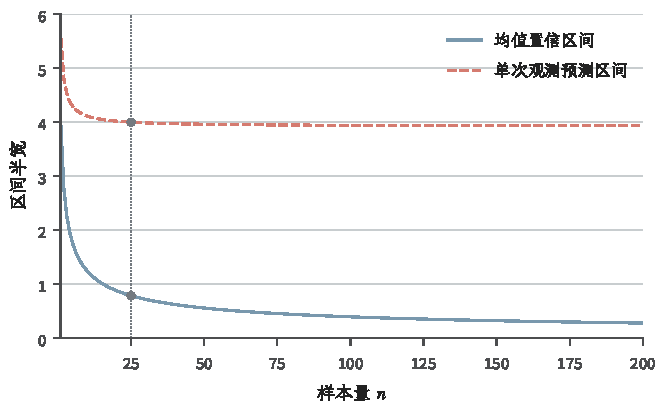
\includegraphics[width=\linewidth]{figures/math-preparation/probability-discrete/statistics-mean-prediction-width.pdf}
  \caption{已知\(\sigma=2\)的独立高斯位置模型中，两类区间半宽随样本量变化（解析式教学图）。使用四舍五入分位数\(1.96\)，蓝实线为\(1.96\sigma/\sqrt n\)，红虚线为\(1.96\sigma\sqrt{1+1/n}\)。灰竖线标出例~\ref{ex:statistics-running-sensor-calibration}的\(n=25\)，没有对任何实测数据重复抽样。}
  \label{fig:statistics-mean-prediction-width}
\end{figure}

\begin{table}[htbp]
  \centering
  \begin{tabular}{p{0.16\linewidth}p{0.29\linewidth}p{0.43\linewidth}}
    \toprule
    类型 & 覆盖对象 & 概率来源与必要条件\\
    \midrule
    置信区间 & 固定总体参数 & 同一抽样制度下重复构造区间的覆盖率\\
    可信区间 & 给定数据的参数后验 & 指定先验与似然形成的后验概率；不自动具有频率覆盖\\
    预测区间 & 尚未观测的随机结果 & 训练样本与未来观测的联合分布；须包含新观测波动\\
    \bottomrule
  \end{tabular}
  \caption{三类区间的覆盖对象与概率来源。区间形式相似时，仍须从所覆盖的对象解释结论。}
  \label{tab:statistics-interval-objects}
\end{table}

方差未知时，用
\[
  S^2=\frac1{n-1}\sum_{i=1}^n(Y_i-\overline Y)^2
\]
估计\(\sigma^2\)。高斯独立样本下，
\[
  \frac{\overline Y-\theta}{S/\sqrt n}\sim t_{n-1},
\]
所以把高斯分位数换成\(t\)分位数可得到精确置信区间。这里的精确性依赖高斯性；
一般分布下它通常只是渐近近似。样本很小且分布偏斜、重尾时，机械使用该区间可能同时
破坏中心和尾部覆盖。

双侧区间与双侧检验在相同模型、显著性水平和统计量下互为反演：若
\(\theta_0\)不在\(1-\alpha\)置信区间内，就拒绝\(H_0:\theta=\theta_0\)。
这种对应关系要求两者使用相同标准误与尾部规则。选择后区间、单侧检验或离散检验中，
不能只凭表面上的阈值照搬这一关系。

\subsubsection{分位数、次序统计量与边际覆盖}

\term{\(q\)分位数}（quantile）可定义为
\[
  F^{-1}(q)=\inf\{y:F(y)\geq q\},\qquad 0<q<1.
\]
这个广义逆为给定的\(F\)和\(q\)选出唯一的下分位数。更一般地，所有满足分位数
不等式的点组成集合
\[
  \mathcal Q_q=\{a:F(a^-)\leq q\leq F(a)\}.
\]
当\(F\)在水平\(q\)上存在平坦区间时，这个集合可能包含多个点；上述广义逆约定选取
其中的下端代表。
对次序统计量\(Y_{(1)}\leq\cdots\leq Y_{(n)}\)，经验分位数由相应秩位置给出。
若\(Y_1,\ldots,Y_n\)是来自连续分布\(F\)的独立同分布样本，则
\(F(Y_{(k)})\)服从
\(\operatorname{Beta}(k,n+1-k)\)，因此可以用秩而不是高斯近似构造分位数区间。
对离散或混合分布，跳跃与平坦区间都要求覆盖计算保留定义中的不等式方向。

总体分位数平均了不同输入；若不同\(x\)对应不同位置或尾部，还需要按输入报告分位数。
\begin{definition}[条件分位数]
  \label{def:statistics-conditional-quantile}
给定\(Y\)关于\(X=x\)的正则条件分布，记\(F_x(y)=\mathbb P(Y\leq y\mid X=x)\)。对\(0<q<1\)，下条件\(q\)分位数为\(F_x^{-1}(q)=\inf\{y:F_x(y)\geq q\}\)；完整条件分位数集合为\(\{a:F_x(a^-)\leq q\leq F_x(a)\}\)。这些对象随条件分布版本确定，并按\(P_X\)-几乎处处意义理解。
\end{definition}
条件分位数可由\term{分位数回归}（quantile regression）估计。假设\(Y\)可积，使下面损失的条件期望对几乎每个\(x\)有限。令
\[
  \rho_q(u)=u\bigl(q-\mathbb{I}_{\{u<0\}}\bigr),
\]
则条件\(q\)分位数最小化
\(\mathbb{E}[\rho_q(Y-a)\mid X=x]\)。固定\(x\)并记条件分布函数为\(F\)，目标对
\(a\)的次梯度区间是
\[
  [F(a^-)-q,\ F(a)-q].
\]
因此最优点恰好满足\(F(a^-)\leq q\leq F(a)\)；连续严格递增时才简化为
\(F(a)=q\)。因此分位数损失的最小点集合正是\(\mathcal Q_q\)，可能不唯一，
而\(F^{-1}(q)\)仍是其中按约定选出的单个代表。分位数回归直接估计条件分布的位置，
不要求误差为高斯或方差恒定。

第~\ref{sec:probability-exchangeability-conformal-ranks}节的共形预测用可交换观测的
秩构造有限样本预测集。具体地，先用与校准集、待预测点分离的训练数据固定评分函数，
再由\(m\)个校准分数\(S_1,\ldots,S_m\)取
\[
  k=\left\lceil(m+1)(1-\alpha)\right\rceil,\qquad
  \widehat q=S_{(k)}.
\]
若\(k=m+1\)，约定阈值为\(+\infty\)；并列分数采用保守的“分数不超过阈值”规则。
校准分数与新分数可交换时，新分数的秩在\(m+1\)个位置上对称，因而分割共形的边际
覆盖结论为
\[
  \mathbb{P}\{Y_{n+1}\in C(X_{n+1})\}\geq1-\alpha.
\]
概率同时平均了不同\(X\)区域。它不推出每个群组或每个
\(x\)都达到同样覆盖率；分组校准只能对预先规定且样本充分的群组提供相应保证，精细到
每个连续条件点的无分布精确覆盖通常不可得。

\subsection{假设检验与误差控制}
\label{sec:statistics-testing-errors}

\subsubsection{检验、p值与区间反演}

区间描述目标的可能范围，\term{假设检验}（hypothesis testing）则检查数据与一个
命题是否相容。
\begin{definition}[随机化检验函数]
  \label{def:statistics-randomized-test-function}
  若单个观测的可测空间为\(\mathcal{Y}\)，则
  \term{随机化检验函数}（randomized test function）是可测映射
  \[
    \varphi:\mathcal{Y}^n\to[0,1].
  \]
  观察到\(\bm{Y}=\bm{y}\)后，检验以概率\(\varphi(\bm{y})\)拒绝原假设。等价地，可另取
  独立的\(U\sim\operatorname{Unif}(0,1)\)，并在
  \(U\leq\varphi(\bm{y})\)时拒绝。只取\(0,1\)值的检验是非随机化特例，其拒绝域为
  \(R=\{\bm{y}:\varphi(\bm{y})=1\}\)。
\end{definition}

原假设\(H_0\)指定被控制误报的情形。检验的大小与参数\(\theta\)下的功效分别为
\[
  \sup_{\theta\in H_0}\mathbb{E}_\theta[\varphi(\bm Y)],
  \qquad
  \mathbb{E}_\theta[\varphi(\bm Y)].
\]
水平为\(\alpha\)要求
\[
  \sup_{\theta\in H_0}
  \mathbb{E}_\theta[\varphi(\bm Y)]
  \leq\alpha.
\]
在\(H_0\)为真时拒绝是第一类错误；在备择\(H_1\)为真时不拒绝是第二类错误。
对非随机化检验，这些期望分别退化为拒绝域概率。效应量描述差异有多大，样本量则影响
能否把该差异从噪声中区分出来。

\term{\(p\)值}（\(p\)-value）是在原假设下，得到至少与当前统计量同样极端结果的
概率。
\begin{definition}[有效p值]
  \label{def:statistics-valid-p-value}
  一个取值于\([0,1]\)的可测统计量\(p(\bm Y)\)是复合原假设\(H_0\)下的有效\(p\)值，若对每个
\(u\in[0,1]\)都有
\[
  \sup_{\theta\in H_0}\mathbb{P}_\theta\{p(\bm Y)\leq u\}\leq u.
\]
\end{definition}
这项零假设下的超均匀性质才保证按阈值\(\alpha\)拒绝时控制第一类错误。观察到的
\(p\)值不是原假设为真的概率，也不是效应量。仍取已知\(\sigma\)的高斯位置模型，
检验\(H_0:\theta=0\)时
\[
  Z=\frac{\sqrt n\,\overline Y}{\sigma},\qquad
  p=2\{1-\Phi(|Z|)\}.
\]
若\(\theta=\delta\)，双侧检验功效为
\[
  \mathbb{P}_\delta(|Z|>z_{1-\alpha/2})
  =
  1-\Phi\left(z_{1-\alpha/2}-\frac{\sqrt n\delta}{\sigma}\right)
  +\Phi\left(-z_{1-\alpha/2}-\frac{\sqrt n\delta}{\sigma}\right).
\]
小样本下“不显著”可能只表示功效不足。相同效应量在更大\(n\)下会得到更小的
\(p\)值。

检验族还可反演为置信集合。对每个候选值\(\theta_0\)，设
\(\varphi_{\theta_0}(\bm Y)\in\{0,1\}\)是水平不超过\(\alpha\)的检验，并定义
\[
  C(\bm Y)=\{\theta_0:\varphi_{\theta_0}(\bm Y)=0\}.
\]
当真实值为\(\theta\)时，
\[
  \mathbb{P}_\theta\{\theta\notin C(\bm Y)\}
  =\mathbb{P}_\theta\{\varphi_\theta(\bm Y)=1\}\leq\alpha,
\]
所以\(C\)具有至少\(1-\alpha\)覆盖率。这里必须对同一模型、同一尾部规则和同一
标准误反演；选择后换检验或只挑有利方向会破坏证明。

\begin{example}[同一效应量下的证据与功效]
\label{ex:statistics-evidence-power-same-effect}
设噪声标准差已知为\(\sigma=2\)，观测均值为\(\overline y=1\)，检验
\(H_0:\theta=0\)。当\(n=4\)时，\(Z=1\)，双侧\(p\)值约为\(0.317\)；
当\(n=100\)时，\(Z=5\)，双侧\(p\)值小于\(10^{-6}\)。两次实验报告的标准化
效应\(\overline y/\sigma=0.5\)相同，证据强度却因标准误不同而变化。

若真实值确为\(\delta=1\)，显著性水平为\(0.05\)，则\(n=4\)时双侧检验功效约为
\[
  1-\Phi(1.96-1)+\Phi(-1.96-1)\approx0.17.
\]
此时未拒绝原假设并不支持“差异为零”。若实际问题把绝对差异不超过\(0.2\)视为等效，
还需要针对\(\Delta=0.2\)设计等效检验；当前样本对这个更严格目标几乎没有辨识力。
\end{example}

\subsubsection{似然比排序与Neyman–Pearson引理}

下面的经典引理给出两个简单假设之间的最强检验\scite{math-lehmann2005testing}
\begin{theorem}[Neyman--Pearson引理]
\label{thm:statistics-neyman-pearson}
对两个完全指定的简单假设\(H_0:P=P_0\)与\(H_1:P=P_1\)，设
\(P_1\ll P_0\)，似然比为\(\Lambda=\mathrm dP_1/\mathrm dP_0\)。在所有大小
不超过\(\alpha\)的检验中，拒绝大似然比并在边界适当随机化的检验具有最大功效。
\end{theorem}

\begin{proof}
取常数\(c\)与边界随机化概率，使检验\(\varphi^\star\)满足
\(\mathbb{E}_0[\varphi^\star]=\alpha\)，并在\(\Lambda>c\)时拒绝、在
\(\Lambda<c\)时接受。对任意\(\mathbb{E}_0[\varphi]\leq\alpha\)的检验，
\[
  (\varphi^\star-\varphi)(\Lambda-c)\geq0
\]
逐点成立，因为\(\varphi^\star\)在\(\Lambda>c\)处取最大允许值，在
\(\Lambda<c\)处取最小允许值。对\(P_0\)积分得到
\[
  \mathbb{E}_1[\varphi^\star-\varphi]
  \geq c\,\mathbb{E}_0[\varphi^\star-\varphi]\geq0.
\]
所以\(\varphi^\star\)的备择拒绝概率不小于任何同大小检验。
\end{proof}

这个结论只直接覆盖两个简单假设。复合假设需要处理未知参数，不一定存在一致最强检验。
在隐私攻击审计中，\(P_0\)与\(P_1\)可分别表示目标记录不在与在训练集时的输出分布；
似然比给出理想攻击排序，但实际审计还要估计这两个分布并计入选择偏差。

\subsubsection{列联表、渐近检验与不同命题}

两个分类变量的列联表中，原假设为独立时，期望格数是
\[
  E_{r,c}=\frac{N_{r,\cdot}N_{\cdot,c}}{N},\qquad
  X^2=\sum_{r,c}\frac{(N_{r,c}-E_{r,c})^2}{E_{r,c}}.
\]
在独立抽样、固定维数且期望格数不过小时，
\(X^2\)近似服从自由度\((R-1)(C-1)\)的卡方分布。稀疏格数会破坏近似，可合并有
科学意义的类别或使用精确、置换方法。条件独立检验还要控制第三个变量；把样本简单切成
大量小层会带来新的稀疏性，不能由普通卡方检验自动解决。

差异检验把“无差异”放在原假设中。等效性检验先给出有实际含义的可接受差异界
\(\Delta>0\)。记\(\delta=\theta_A-\theta_B\)，两个单侧检验（two one-sided
tests, TOST）把不等效原假设写成两个集合的并：
\[
  H_0=H_{0,L}\cup H_{0,U},
  \qquad
  H_{0,L}:\delta\leq-\Delta,
  \qquad
  H_{0,U}:\delta\geq\Delta.
\]
对应备择为\(-\Delta<\delta<\Delta\)。TOST只有在水平\(\alpha\)的下侧检验拒绝
\(H_{0,L}\)，并且水平\(\alpha\)的上侧检验也拒绝\(H_{0,U}\)时，才拒绝总体原假设。
例如，若\(\widehat\delta\)的标准误为\(s\)，且标准化统计量服从相应正态近似，
拒绝条件为
\begin{equation}
  \frac{\widehat\delta+\Delta}{s}>z_{1-\alpha}
  \quad\text{且}\quad
  \frac{\widehat\delta-\Delta}{s}<z_{\alpha}.
  \label{eq:statistics-tost-rejection}
\end{equation}
这等价于把双侧\(1-2\alpha\)置信区间完整放入
\((-\Delta,\Delta)\)。总体第一类错误并非\(2\alpha\)：只要
\(\delta\in H_0\)，至少有一个单侧原假设为真，而总体拒绝事件包含在拒绝这个真原假设
的事件中，所以其概率至多为\(\alpha\)。非劣效检验只排除一个方向，例如
\(H_0:\delta\leq-\Delta\)。未拒绝差异检验的零假设不等于证明等效。

\subsection{重采样与经验不确定性}
\label{sec:statistics-resampling}

\subsubsection{Bootstrap与抽样分布近似}

复杂估计量的抽样分布难以解析计算时，可以让经验数据模拟重复抽样。
\term{Bootstrap}从经验分布
\(\widehat P_n=n^{-1}\sum_i\Delta_{Y_i}\)有放回抽取\(n\)个观测，并重新计算
\(\widehat\tau^\ast\)。条件于原样本的
\(\widehat\tau^\ast-\widehat\tau\)近似
\(\widehat\tau-\tau(P)\)的抽样波动。简单百分位区间取Bootstrap估计值的经验分位数，
但对不光滑统计量、边界参数、极端尾部分位数或重尾小样本，近似可能很差。

对独立同分布、方差\(0<\sigma^2<\infty\)的样本均值，这个近似有清楚的缩放口径。
若\(\overline Y^\ast\)由经验分布条件重抽样，则下述条件分布依概率弱收敛：
\[
  \mathcal L\!\left(
    \sqrt n(\overline Y^\ast-\overline Y)\mid\bm Y
  \right)
  \Longrightarrow\mathcal N(0,\sigma^2),
\]
与\(\sqrt n(\overline Y-\mu)\)的极限相同。经验均值等于\(\overline Y\)，经验方差
依概率趋于\(\sigma^2\)，但方差收敛本身还不足以保证条件中心极限定理。有限二阶矩还使
每个\(\varepsilon>0\)对应的条件Lindeberg尾项满足
\[
  \frac1n\sum_{i=1}^n(Y_i-\overline Y)^2
  \mathbb I\{|Y_i-\overline Y|>\varepsilon\sqrt n\}
  \xrightarrow{\mathbb P}0.
\]
这表示单个极端观测不会贡献不可忽略的总方差：\(\overline Y\to\mu\)，而有限二阶矩
使越来越远的平方尾部积分趋于零。对给定原样本后独立的重抽样应用三角阵列中心极限定理，
便得到上述条件极限。该结论针对中心化、缩放后的条件分布；它本身不自动证明任意百分位
区间具有高阶准确性。

例~\ref{ex:statistics-running-sensor-calibration}中的经验分布均值为\(10.4\)，经验
方差按分母\(n\)计算恰为\(4\)。因此单次Bootstrap抽样值满足
\[
  \mathbb{E}_\ast[Y^\ast]=10.4,\qquad
  \operatorname{Var}_\ast(Y^\ast)=4,
\]
而二十五次有放回抽样的均值满足
\[
  \operatorname{SE}_\ast(\overline Y^\ast)
  =
  \sqrt{\frac4{25}}=0.4.
\]
若中心化并按标准误标准化后的条件Bootstrap分布可由标准正态分布近似，则正态
Bootstrap区间为
\(10.4\pm1.96\times0.4=[9.62,11.18]\)，与已知方差高斯区间在这个构造例中重合。
重合来自经验方差刚好等于已知噪声方差以及均值的光滑性，不是Bootstrap总会复制参数
区间的保证。

这种近似可由平滑统计泛函的线性化理解。若
\[
  \widehat\tau-\tau(P)
  =
  \frac1n\sum_{i=1}^n\operatorname{IF}(Y_i;T,P)
  +o_{\mathbb{P}}(n^{-1/2}),
\]
那么Bootstrap样本条件于原数据也产生相同形式的一阶平均，只是把\(P\)替换成
\(\widehat P_n\)。因此两边经\(\sqrt n\)缩放后的分布接近。样本最大值之类统计量
没有这种常规线性展开：经验分布不会生成比当前最大值更大的观测，简单Bootstrap便可能
错误描述尾部。

\subsubsection{置换与零假设随机化}

\term{置换检验}（permutation test）近似的不是估计量抽样分布，而是零假设下标签可
交换时的随机化分布。两组观测在“处理标签不影响联合分布”的原假设下，可反复打乱标签
并重算组间差异。若分配机制只允许在区组内交换，就必须在区组内置换；任意全局打乱会
制造实验中不可能出现的分配。

若允许的置换集合有\(M\)个元素，并把观测统计量与全部置换统计量一起排序，则交换
对称性使真实排列的秩在这些位置上均匀；存在并列时使用
\[
  p_{\mathrm{perm}}
  =\frac{\#\{\text{置换统计量不小于观测值}\}}{M}
\]
得到超均匀而可能保守的\(p\)值。若只随机抽取\(B\)个置换，常用
\((1+\#\{\text{抽样置换不小于观测值}\})/(B+1)\)保留有限模拟下的保守性。
仅有两组均值相等并不保证整批标签可交换；交换性必须来自更强的零假设或随机分配设计。

重采样单位必须跟独立单位一致。配对实验对整对数据重采样；多个记录属于同一用户时对
用户群组重采样；时间相关数据使用保留局部依赖的块Bootstrap。逐条重采样会把共享噪声
误当作独立波动，通常低估标准误。

\subsection{选择、多重比较与持续查看}
\label{sec:statistics-selection-multiplicity}

\subsubsection{多个假设与选中候选}

单个检验的第一类错误为\(\alpha\)，不代表同时尝试许多候选后仍只有
\(\alpha\)的误报概率。若\(m\)个原假设都为真，联合界给出
\[
  \mathbb{P}(\text{至少一次误拒绝})
  \leq\sum_{j=1}^m\mathbb{P}(\text{拒绝 }H_j)
  \leq m\alpha.
\]
Bonferroni方法把每项阈值设为\(\alpha/m\)，从而控制
\term{族错误率}（family-wise error rate, FWER）。它不要求检验独立，但候选很多时
可能保守。

Holm方法把\(p\)值从小到大排序，并依次将
\(p_{(j)}\)与\(\alpha/(m-j+1)\)比较，遇到第一个未拒绝项即停止。若第一个被错误
拒绝的真原假设位于位置\(j\)，设真原假设总数为\(m_0\)，则前\(j-1\)项均为假
原假设，所以\(m-j+1\geq m_0\)。该真原假设的\(p\)值因而不超过
\(\alpha/(m-j+1)\leq\alpha/m_0\)。对全部\(m_0\)个真原假设应用联合界，便把
发生任一错误拒绝的概率控制在\(\alpha\)以内。它与Bonferroni一样不要求独立，但利用
了逐步比较。

当目标是控制所有拒绝中错误发现的期望比例时，可使用
\term{错误发现率}（false discovery rate, FDR）。设\(R\)为拒绝的总数、\(V\)为其中
被错误拒绝的真原假设数，则
\[
  \operatorname{FDR}=\mathbb E\left[\frac{V}{\max(R,1)}\right].
\]
当\(R=0\)时，错误发现比例约定为零；这是随机比例的期望，不是
\(\mathbb EV/\mathbb ER\)。Benjamini--Hochberg过程将
\(p\)值排序为\(p_{(1)}\leq\cdots\leq p_{(m)}\)，找最大
\[
  k=\max\left\{j:p_{(j)}\leq\frac{j}{m}q\right\},
\]
并拒绝前\(k\)项；若集合为空，则取\(k=0\)，不拒绝任何假设。若全部\(p\)值相互
独立，且每个真原假设下的\(p\)值满足
\(\mathbb P(p_j\leq u)\leq u\)（\(0\leq u\leq1\)），该过程控制FDR不超过目标
\(q\in(0,1)\)\scite{statistics-benjamini-hochberg1995}扩展到依赖检验需要更精确的联合分布条件，不能仅凭两两正相关或任意
依赖就沿用这项保证。

从多个模型中挑选测试误差最小者，再把该最小值当成固定模型的无偏评估，会系统性偏乐观。
候选越多，偶然低估越容易被选中。解决办法是把选择和最终评价分开，或把“选择算法”
整体作为待评价对象。固定模型的区间不能在选择后继续冒充选中模型的区间。

例~\ref{ex:statistics-running-sensor-calibration}还需要从两个预先给定的带宽中选择一个。
用一个刻意简化、可精确计算的噪声模型说明选择偏差：假设两个带宽的真实预测均方误差都
是\(4\)，验证误差分别为
\[
  \widehat R_j=4+\varepsilon_j,\qquad
  \mathbb{P}(\varepsilon_j=0.8)
  =\mathbb{P}(\varepsilon_j=-0.8)=\frac12,
  \quad j=1,2,
\]
并且两个误差独立。每个\(\widehat R_j\)单独都是无偏的，但两者最小值以概率
\(1/4\)等于\(4.8\)，以概率\(3/4\)等于\(3.2\)，所以
\[
  \mathbb{E}\min(\widehat R_1,\widehat R_2)
  =\frac14\times4.8+\frac34\times3.2
  =3.6.
\]
把选中带宽的\(3.6\)当作未来风险，平均会低估\(0.4\)。嵌套交叉验证或独立测试集的
作用，是评价“比较两个带宽再选择”这一完整流程，而不是重新评价已知固定的单个带宽。

\subsubsection{交叉验证与流程评价}

\term{交叉验证}（cross-validation）把数据轮流分成训练部分和验证部分，估计“用同样
训练流程在新数据上的预测误差”。它同时依赖训练规模、划分单位和调参流程。若用同一组
折选择超参数又报告最优分数，结果仍含选择乐观偏差；需要嵌套交叉验证或独立测试集评估
整个选择流程。

交叉验证各折的误差也不是彼此独立，因为训练集大量重叠。因此不能把\(K\)个折分数当成
\(K\)个独立观测，再用普通样本方差构造过窄区间。若目标是比较两个算法，应在相同划分
上计算配对差异，并把数据集抽样和训练随机性纳入评价设计；单次\(K\)折结果主要用于
误差估计与模型选择，不自动提供精确的显著性检验。

\subsubsection{持续查看与停止规则}

持续查看同一数据也构成选择。固定时刻满足
\(\mathbb{P}(p_t\leq\alpha)\leq\alpha\)并不推出
\(\mathbb{P}(\exists t:p_t\leq\alpha)\leq\alpha\)。预先规定查看次数可分配
\(\alpha\)预算；更灵活的停止规则需要序贯检验、置信序列或由非负超鞅构造的
\(e\)值。停止规则属于推断程序的一部分，不能在看到结果后删去。

定义~\ref{def:stoch-confidence-sequence}的\term{置信序列}（confidence sequence）把所有时刻的覆盖放在同一个高概率事件中。这比每个固定时刻各自覆盖更强，因为允许依据当前数据决定何时停止查看。
若\((E_t)\)在原假设下是从\(E_0=1\)开始的非负超鞅，则Ville不等式给出
\[
  \mathbb{P}_0\left\{\sup_{t\geq0}E_t\geq\frac1\alpha\right\}\leq\alpha.
\]
因此可以在任意由过去信息决定的停止时刻按阈值查看\(E_t\)，而不增加这项越界概率。
这不表示停止后的点估计无偏，也不表示同时尝试多个证据过程无需额外控制；覆盖、估计
偏差和模型选择证据仍是不同问题。

\section{概率预测与非参数表示}
\label{sec:stats-prediction-observation-limits}

推断也可以以未来观测的分布为目标，而不只估计一个有限维参数。评分与校准评价所给出的概率，
非参数方法则放宽分布形状假设，用局部数据构造密度或预测函数。
本节分别说明如何评价这个目标，以及更灵活的表示怎样带来带宽与邻域的选择问题；
它们仍复用本章开头的抽样和观测机制条件。

\subsection{概率预测、评分与校准}
\label{sec:statistics-scoring-calibration}

\subsubsection{适当评分与最优预测分布}

点预测只给一个结果，概率预测则给出整个候选分布。若只奖励是否猜中最可能结果，报告完整概率并没有优势；评分必须鼓励把真实不确定性如实报告。
\begin{definition}[适当评分规则]
  \label{def:statistics-proper-scoring-rule}
  给定预测分布类\(\mathcal P\)，\term{评分规则}（scoring rule）\(S(Q,y)\)，即报告预测分布\(Q\)而结果为\(y\)
时承担的损失。假定所比较的期望均有定义，且诚实报告的期望有限。若对每个\(P,Q\in\mathcal P\)有\(\mathbb E_PS(P,Y)\leq\mathbb E_PS(Q,Y)\)，就称评分规则
\term{适当}（proper）；若适用分布类中的最小点唯一，则称为严格适当。
\end{definition}
它奖励诚实概率，而不是只检查最可能类别是否猜中。

先考虑有限结果集\(\mathcal Y\)，并记\(P,Q\)的概率质量函数为\(p,q\)。本节只需
有限离散情形的\term{KL散度}（Kullback--Leibler divergence）：
\[
  D_{\mathrm{KL}}(P\Vert Q)
  =
  \sum_{y\in\mathcal Y}p(y)\log\frac{p(y)}{q(y)}.
\]
其中约定\(0\log(0/q)=0\)；只要存在\(p(y)>0\)而\(q(y)=0\)，就令散度为
\(+\infty\)。由\(-\log u\geq1-u\)可得
\(D_{\mathrm{KL}}(P\Vert Q)\geq0\)，等号当且仅当\(P=Q\)。
这也可看成对凸函数\(-\log\)应用Jensen不等式：在\(P\)的支持上平均
\(q(y)/p(y)\)，所得总和不超过\(1\)。
第~\ref{chap:information-theory-and-statistical-geometry}章将在一般测度空间上定义
这一量，并系统讨论其性质。

离散结果的对数评分为\(S(Q,y)=-\log q(y)\)。根据上述定义，其期望差满足
\[
  \mathbb{E}_P[S(Q,Y)]-\mathbb{E}_P[S(P,Y)]
  =\sum_{y\in\mathcal Y}p(y)\log\frac{p(y)}{q(y)}
  =D_{\mathrm{KL}}(P\Vert Q)\geq0.
\]
因此对数评分是严格适当的；零预测概率遗漏真实分布的支持时，期望损失为无穷。
连续密度版本还要求相对于共同参考测度定义密度，并保证相关对数期望有定义；改变参考
坐标会改变单个对数密度值，但在合法换元下比较同一结果分布的期望差保持一致。

二元结果\(Y\in\{0,1\}\)的Brier评分为\(S(q,Y)=(q-Y)^2\)。若真实事件概率为
\(p\)，则
\begin{align}
  \mathbb{E}_p[(q-Y)^2]
  &=p(q-1)^2+(1-p)q^2\\
  &=(q-p)^2+p(1-p).
\end{align}
第二项与报告\(q\)无关，所以唯一最优报告是\(q=p\)。对数评分更强烈惩罚对已发生
事件给极小概率，Brier评分则有界；两者表达不同风险偏好。

对\(K\)个类别，令真实概率向量为\(\bm p\)，报告为\(\bm q\)，Brier评分可写成
\(S(\bm q,Y)=\sum_{k=1}^K(q_k-\mathbb{I}\{Y=k\})^2\)。直接展开得到
\[
  \mathbb{E}_{\bm p}[S(\bm q,Y)]
  =\lVert\bm q-\bm p\rVert_2^2
   +1-\lVert\bm p\rVert_2^2.
\]
所以它在概率单纯形上同样严格适当，但控制的是概率向量的平方距离，不是对数密度比。

\subsubsection{校准、区分能力与锐度}

\begin{definition}[二元概率校准]
  \label{def:statistics-probability-calibration}
  设\(Y\in\{0,1\}\)，预测概率为随机变量\(Q\in[0,1]\)。若
  \[ \mathbb E[Y\mid Q]=Q\quad\text{几乎必然}, \]
  则称预测相对于当前联合总体分布是\term{校准}（calibration）的。等价地，\(\mathbb P(Y=1\mid Q=q)=q\)对\(P_Q\)-几乎每个\(q\)成立。
\end{definition}
它要求预测概率相同的一组样本具有相应的真实发生率，而不要求有限样本中每组频数恰好等于预测值。\term{区分能力}（discrimination）描述模型
能否给更可能发生事件的样本更高分；\term{锐度}（sharpness）描述预测分布是否集中。
对所有样本恒报基准发生率可以完美校准，却没有区分能力。锐度只有在校准前提下才值得
追求。

令\(Q=\widehat p(X)\)、\(\eta(Q)=\mathbb{E}[Y\mid Q]\)，再记总体发生率为
\(\overline p=\mathbb{E}[Y]\)。条件平方展开给出
\[
  \mathbb{E}[(Q-Y)^2]
  =
  \underbrace{\mathbb{E}[(Q-\eta(Q))^2]}_{\text{校准误差}}
  +\underbrace{\overline p(1-\overline p)
    -\operatorname{Var}(\eta(Q))}_{\text{剩余不可分辨误差}}.
\]
第一项为零才表示相对于预测值本身校准；第二项随不同预测组的真实风险更可区分而减小。
恒报\(\overline p\)使第一项为零，却也使
\(\operatorname{Var}(\eta(Q))=0\)。多类别校准相应要求
\(\mathbb{P}(Y=k\mid\widehat{\bm p})=\widehat p_k\)对每个类别成立，逐类别边际校准
通常弱于这个向量条件。

一个固定的两组例子可以把这几个性质分开。设两组各占总体一半，事件概率分别为\(0.2,0.8\)。如表~\ref{tab:statistics-calibration-discrimination}，恒报\(0.5\)和按组报\(0.2,0.8\)都校准；前者把两组混在一起，后者保留了风险差异。按组报\(0,1\)保持相同排序，预测更集中，却把仍可能发生的意外结果说成不可能。
\begin{table}[htbp]
  \centering
  \small
  \begin{tabular}{lccc}
    \toprule
    报告规则 & 两组概率 & 总体校准 & 期望Brier损失 \\
    \midrule
    恒报总体发生率 & \(0.5,0.5\) & 是 & \(0.25\) \\
    如实报告组风险 & \(0.2,0.8\) & 是 & \(0.16\) \\
    只保留确定类别 & \(0,1\) & 否 & \(0.20\) \\
    \bottomrule
  \end{tabular}
  \caption{同一个两组总体下的校准与区分能力。数值由\(\mathbb E[(q-Y)^2]=(q-p)^2+p(1-p)\)逐组平均得到；后两行的类别排序相同，但概率准确性不同。}
  \label{tab:statistics-calibration-discrimination}
\end{table}

\subsubsection{后处理校准与评价条件}

温度缩放对分类logit \(\bm z\)使用
\(\operatorname{softmax}(\bm z/T)\)，在校准集上按对数损失估计\(T>0\)。它保持
类别排序，只调整置信程度。保序回归则拟合单调的分数到概率映射，更灵活但更容易在小
校准集上过拟合。给定排序分数\(s_i\)，其典型拟合问题是在
\(q_1\leq\cdots\leq q_m\)约束下最小化
\(\sum_i(q_i-y_i)^2\)；单调约束不等于总体校准保证。
训练原预测器、拟合校准器和评价校准效果应使用职责分离的数据或严格的折外预测；
部署总体若发生变化，旧映射也未必保持校准。分箱可靠性图只是把连续条件近似成有限组，
箱内比例仍有抽样误差，且结果依赖分箱边界。适当评分、边际覆盖和校准分别评价分布损失、
未来集合与条件发生率，不能互相替代。

\subsection{非参数估计}
\label{sec:statistics-nonparametric-missing}

\subsubsection{密度估计与带宽}

有限维模型可能把真实分布限制得过强。非参数方法不预先固定有限个参数，但仍通过带宽、
邻域或平滑度控制复杂度。以下令\(Y_1,\ldots,Y_n\)独立同分布，具有同一个一维
密度\(f\)，并采用不依赖本批观测的带宽\(h=h_n>0\)。相关、选择或加权样本
需要另行计算期望与协方差，不能直接使用下面的独立样本公式。给定宽度为\(h\)的分箱，直方图用
“箱内样本数除以\(nh\)”作为箱内常数密度；移动箱边界可能改变估计。核密度估计则把
每个样本扩散为核：
\[
  \widehat f_h(x)
  =\frac1{nh}\sum_{i=1}^n
    K\left(\frac{x-Y_i}{h}\right).
\]
若\(K\geq0\)、积分为\(1\)，则\(\widehat f_h\)本身是非负且积分为\(1\)的密度。
为直接使用局部Taylor展开，以下采用一组充分条件：\(K\)有界、紧支撑且对称，
二阶矩记为\(\mu_2(K)=\int u^2K(u)\,\mathrm du\)，并记
\(R(K)=\int K(u)^2\,\mathrm du\)；两者均有限。设\(f\)在内部点\(x\)的邻域
二阶连续可微，则小带宽下核只涉及这个光滑邻域，由
\[
  \mathbb{E}[\widehat f_h(x)]
  =\int K(u)f(x-hu)\,\mathrm du
\]
作Taylor展开，核的一阶矩因对称性消失，从而得到
\[
  \operatorname{Bias}\{\widehat f_h(x)\}
  =\frac{h^2\mu_2(K)}2f''(x)+o(h^2),
\]
\[
  \operatorname{Var}\{\widehat f_h(x)\}
  =\frac{f(x)R(K)}{nh}+o((nh)^{-1}),
\]
其中渐近式取\(h\to0\)、\(nh\to\infty\)。较大带宽降低方差却增加平滑偏差。
边界附近因核质量落到支持集外，上述对称展开失效。
在\(d\)维中，体积因子变为\(h^d\)，代表性点态方差阶数相应为
\(1/(nh^d)\)。因此维数增加会更快消耗局部样本；一维的带宽结论不能不改条件直接
移植到高维。

\subsubsection{局部预测与近邻}

这里的观测改为\((X_i,Y_i)_{i=1}^n\)，假定它们来自同一联合分布且独立同分布，
\(Y\)可积。采用上一小节的非负、有界、紧支撑核\(K\)与确定带宽\(h>0\)。
回归函数\(m(x)=\mathbb{E}[Y\mid X=x]\)可由局部平均估计；以下比值只在
权重和\(\sum_iK((X_i-x)/h)>0\)时定义：
\[
  \widehat m_h(x)=
  \frac{\sum_iK((X_i-x)/h)Y_i}
       {\sum_iK((X_i-x)/h)}.
\]
局部线性回归在\(x\)附近拟合\(a+b(X_i-x)\)，在相应平滑条件下可减轻设计
密度不均和边界偏差。下面的唯一拟合还要求局部加权设计满秩；在这个一维两参数问题中，
即正权重的输入至少含两个不同取值。若权重和为零或设计退化，需扩大邻域或另给退化处理，
不能照用比值或逆矩阵公式。
\[
  (\widehat a,\widehat b)
  \in\argmin_{a,b}\sum_{i=1}^n
  K\left(\frac{X_i-x}{h}\right)
  \{Y_i-a-b(X_i-x)\}^2,
  \qquad \widehat m_{\mathrm{local}}(x)=\widehat a.
\]
\(k\)近邻取\(1\leq k\leq n\)，用离\(x\)最近的\(k\)个样本平均；距离并列时
按预先指定的规则选择。维数增大时，为包含足够邻居必须扩大
邻域，Taylor局部性随之变差，这就是维数灾难的一种表现。

在例~\ref{ex:statistics-running-sensor-calibration}的左边界\(x_0=0\)，局部常数
估计为
\[
  \widehat m_h(0)
  =
  \frac{1\times9+0.75\times11+0.25\times13}
       {1+0.75+0.25}
  =10.25.
\]
局部线性拟合令\(u_i=x_i-x_0\)。由这三个点可算得
\[
  S_0=\sum_i w_i=2,\quad
  S_1=\sum_i w_i u_i=1.5,\quad
  S_2=\sum_i w_i u_i^2=3,
\]
\[
  T_0=\sum_i w_i y_i=20.5,\qquad
  T_1=\sum_i w_i u_i y_i=18.
\]
加权正规方程给出
\[
  \widehat a
  =\frac{S_2T_0-S_1T_1}{S_0S_2-S_1^2}
  =9.2,\qquad
  \widehat b
  =\frac{S_0T_1-S_1T_0}{S_0S_2-S_1^2}
  =1.4.
\]
因此局部线性预测为\(9.2\)，而局部常数预测为\(10.25\)。在边界处，后者只能对单侧
观测加权平均，前者还估计局部斜率并把直线截距放回\(x_0\)；哪一个更接近真实条件均值
仍取决于局部线性近似和带宽是否合适，不能由这一组数值单独决定。

图~\ref{fig:statistics-local-boundary-fit}显示这两个预测值的几何区别：水平线只改变高度，斜线同时解释输入位置与响应的局部变化，再把截距取回边界点。图中的观测和权重就是上面的三个教学数据；未画出未知的真实条件均值，因此不能从图上断言哪一种估计误差更小。
\begin{figure}[htbp]
  \centering
  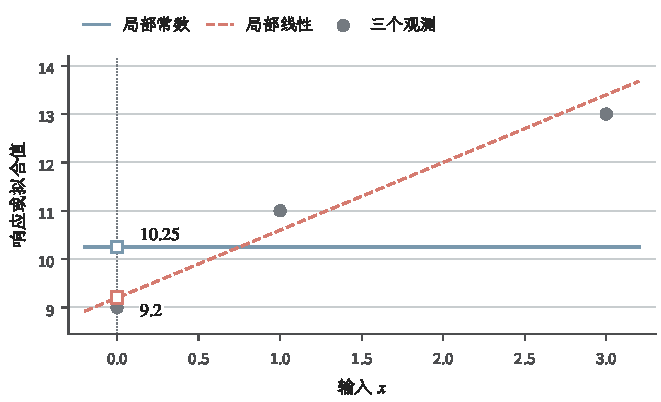
\includegraphics[width=\linewidth]{figures/math-preparation/concept-revision-probability/statistics-local-boundary-fit.pdf}
  \caption{边界处的局部常数与局部线性拟合（教学数据图）。观测为\((0,9),(1,11),(3,13)\)，权重为\(1,0.75,0.25\)。蓝实线为加权常数\(10.25\)，红虚线为\(9.2+1.4x\)，边界\(x_0=0\)处分别预测\(10.25\)和\(9.2\)。}
  \label{fig:statistics-local-boundary-fit}
\end{figure}

在上述独立同分布抽样下，这些方法的一致性需要邻域既缩小又包含越来越多样本。
例如一维内部点处，若输入密度在
\(x\)附近连续且为正，条件均值足够光滑，条件方差局部有界，并取
\(h\to0\)、\(nh\to\infty\)，局部常数估计的平滑偏差消失，局部平均的方差也消失。
输入密度与条件均值都二阶连续可微时，常用局部展开给出\(O(h^2)\)的平滑偏差
以及\(O((nh)^{-1})\)的方差，因此平滑偏差的平方为\(O(h^4)\)；精确常数还依赖
核、输入密度与条件噪声。近邻版本相应要求\(k\to\infty\)且\(k/n\to0\)。
这些都是目标分布有局部覆盖时的内插结论；在训练输入密度为零的区域，缩小邻域无法产生
新信息，外推保证必须来自额外结构假设。

\section{模型比较与数据获取}
\label{sec:stats-model-comparison-data-acquisition}

当一个模型或一批数据不足以回答问题时，有两种决策需要区分：用现有数据比较候选模型，
以及通过新的对照或观测增加信息。模型证据需要统一比较口径；实验设计需要说明新增数据
将减少哪一项不确定性。二者都使用前面的推断工具，却改变不同的决策对象。

\subsection{模型证据与局部积分近似}
\label{sec:statistics-model-evidence}

上一组工具评价预测分布；多个模型竞争时，还需先决定比较的是训练拟合、未来预测还是模型证据。
边缘似然对参数积分，Laplace近似用局部曲率近似这项积分。
信息准则的惩罚形式虽可能相似，比较目标和渐近条件却不同。

\subsubsection{预测、似然与边缘似然}

模型选择准则并非都在回答同一问题。独立测试误差比较未来预测；训练似然衡量已观测数据
在拟合参数下的密度；边缘似然
\[
  p(\bm y\mid M)
  =\int p(\bm y\mid\vartheta,M)\pi(\vartheta\mid M)\,\mathrm d\vartheta
\]
对参数不确定性积分；编码长度则把模型和数据的描述代价相加。一个模型可能训练似然高，
却因复杂度、先验体积或泛化误差而不被其他准则选择。

\begin{definition}[Bayes因子]
  \label{def:statistics-bayes-factor}
两个模型\(M_1,M_0\)的\term{Bayes因子}（Bayes factor）是
\[
  \operatorname{BF}_{1,0}
  =\frac{p(\bm y\mid M_1)}{p(\bm y\mid M_0)}.
\]
这里两个边缘似然都由概率先验得到；所比较的数据处，分母严格为正且有限，分子有限且可为零。
\end{definition}
Bayes因子更新的是模型间先验赔率，
不是与先验无关的“模型为真概率”。在高斯位置模型中，若
\(\theta\sim\mathcal N(0,A^2)\)，则
\(\overline Y\sim\mathcal N(0,A^2+\sigma^2/n)\)。保持似然峰值不变而增大\(A\)
会把先验质量摊到更宽区域；对固定\(\overline y\)，当\(A\to\infty\)时该边缘密度
趋于零。这正是模型证据依赖参数先验尺度的一个可复核例子。

\subsubsection{Laplace近似与BIC}

\begin{theorem}[固定维Laplace局部积分近似]
\label{thm:statistics-laplace-approximation}
设\(\Theta\subseteq\mathbb{R}^d\)为可测集，
\(\widehat{\bm\vartheta}\in\operatorname{int}(\Theta)\)。函数
\(h:\Theta\to\mathbb{R}\)可测，并在
\(\widehat{\bm\vartheta}\)的某个邻域内二阶连续可微；该点是\(h\)在\(\Theta\)上的
唯一全局最大点，且
\(\bm H=-\nabla^2h(\widehat{\bm\vartheta})\)正定。函数
\(g:\Theta\to[0,\infty)\)局部可积，在该点的某个邻域内连续，并满足
\(g(\widehat{\bm\vartheta})>0\)。

进一步假设存在\(\delta,\eta>0\)和\(n_0\geq1\)，使
\(\overline{B_\delta(\widehat{\bm\vartheta})}\subseteq\Theta\)，\(h,g\)在该闭球
所在的邻域内分别满足上述光滑性与连续性，并且
\[
  \sup_{\bm\vartheta\in
    \Theta\setminus B_\delta(\widehat{\bm\vartheta})}
  h(\bm\vartheta)
  \leq h(\widehat{\bm\vartheta})-\eta,
  \qquad
  \int_\Theta
  \exp\!\left\{n_0\bigl[h(\bm\vartheta)
    -h(\widehat{\bm\vartheta})\bigr]\right\}
  g(\bm\vartheta)\,\mathrm d\bm\vartheta<\infty.
\]
则当\(n\to\infty\)时，
\[
  \int_\Theta \exp\{n h(\bm\vartheta)\}g(\bm\vartheta)\,
  \mathrm d\bm\vartheta
  =
  \exp\{nh(\widehat{\bm\vartheta})\}
  g(\widehat{\bm\vartheta})
  \left(\frac{2\pi}{n}\right)^{d/2}
  |\bm H|^{-1/2}\{1+o(1)\}.
\]
\end{theorem}

\begin{proof}
正定性与二阶连续性保证：必要时缩小\(\delta\)，存在\(c>0\)，使闭球内有
\[
  h(\bm\vartheta)-h(\widehat{\bm\vartheta})
  \leq-c\lVert\bm\vartheta-\widehat{\bm\vartheta}\rVert_2^2.
\]
缩小闭球后，原闭球中剩余的紧致环带由唯一最大性给出严格间隔；把它与原来的尾部间隔
合并，仍可取某个\(\eta>0\)满足定理中的一致上界。另一方面，在最大点附近作多元
Taylor展开：
\[
  h(\bm\vartheta)
  =
  h(\widehat{\bm\vartheta})
  -\frac12(\bm\vartheta-\widehat{\bm\vartheta})^\top
  \bm H(\bm\vartheta-\widehat{\bm\vartheta})
  +o(\lVert\bm\vartheta-\widehat{\bm\vartheta}\rVert_2^2).
\]
令
\(\bm u=\sqrt n\,\bm H^{1/2}
(\bm\vartheta-\widehat{\bm\vartheta})\)，则逆变换的Jacobian行列式绝对值为
\(n^{-d/2}|\bm H|^{-1/2}\)，即
\(\mathrm d\bm\vartheta
=n^{-d/2}|\bm H|^{-1/2}\mathrm d\bm u\)。对每个固定的\(\bm u\)，
Taylor展开与\(g\)的连续性
使变换后的被积函数收敛到
\(g(\widehat{\bm\vartheta})\exp(-\lVert\bm u\rVert_2^2/2)\)。局部二次上界和
\(g\)在闭球上的有界性给出可积的高斯控制函数，因此支配收敛定理给出
\[
  \int_{B_\delta(\widehat{\bm\vartheta})}
  \exp\!\left\{n\bigl[h(\bm\vartheta)
    -h(\widehat{\bm\vartheta})\bigr]\right\}
  g(\bm\vartheta)\,\mathrm d\bm\vartheta
  =
  n^{-d/2}|\bm H|^{-1/2}
  g(\widehat{\bm\vartheta})(2\pi)^{d/2}\{1+o(1)\}.
\]
闭球外的尾项满足
\[
  \int_{\Theta\setminus B_\delta(\widehat{\bm\vartheta})}
  e^{n[h(\bm\vartheta)-h(\widehat{\bm\vartheta})]}
  g(\bm\vartheta)\,\mathrm d\bm\vartheta
  \leq
  e^{-(n-n_0)\eta}
  \int_\Theta
  e^{n_0[h(\bm\vartheta)-h(\widehat{\bm\vartheta})]}
  g(\bm\vartheta)\,\mathrm d\bm\vartheta
  =o(n^{-d/2}).
\]
局部主项与该尾项相加即得结论。
\end{proof}

上一定理描述固定函数\(h\)的基本形式。在正则独立样本模型中，实际处理的是随机函数
序列
\[
  nh_n(\bm\vartheta)=\ell_n(\bm\vartheta)
  =\sum_{i=1}^n\log p_\vartheta(y_i),\qquad
  g(\bm\vartheta)=\pi(\bm\vartheta).
\]
若极大似然估计以内点唯一最大点的形式收敛，归一化观测信息矩阵收敛到正定极限，先验
在极限点附近连续且为正，并且局部二次展开与尾部控制对该序列一致成立，则相同论证给出
\[
  \log p(\bm y\mid M)
  =
  \ell_n(\widehat{\bm\vartheta})
  -\frac d2\log n+O_{\mathbb{P}}(1).
\]
对固定的有限候选模型集合，乘以\(-2\)并只保留随\(n\)发散的项，得到常用形式
\[
  \operatorname{BIC}
  =-2\ell_n(\widehat{\bm\vartheta})+d\log n.
\]
惩罚来自后验高密度区域体积随\(n^{-d/2}\)缩小，而不是人为给参数个数加价。

\subsubsection{AIC、描述长度与比较口径}

在独立、固定维且正则的最大似然设定中，常用
\[
  \operatorname{AIC}
  =-2\ell_n(\widehat{\bm\vartheta})+2d.
\]
其中\(2d\)是一阶校正拟合对预期样本外对数损失的乐观偏差，目标是预测失配；模型失配
时还要核对适用的协方差校正，不能只数参数。BIC近似特定先验下的边缘似然，常以候选中
存在真模型的正则渐近为背景。\term{最小描述长度}（minimum description length,
MDL）则先规定可解码的模型代码与给定模型后的数据代码，再最小化二者总长度；更换编码
对象或精度约定会改变有限样本准则。三者惩罚形式相似时也不能互换解释，更不能共享未经
证明的选择一致性。

混合模型的标签交换、参数位于边界、额外成分权重为零或Fisher信息奇异时，最大点可能
不唯一，局部曲率可能退化，常规Laplace展开和\(d\log n\)惩罚随之失效。此时应使用
适合奇异模型的方法、数值积分或明确的近似；近似边缘似然不能写成精确证据。

\subsection{对照、预算与信息获取}
\label{sec:statistics-design-information}

\subsubsection{随机分配与可复核对照}

推断质量不仅由分析方法决定，也由数据如何取得决定。每个对象在各处理下本会产生的结果
称为潜在结果，正式的因果目标将在第~\ref{chap:causal-inference}章定义。随机分配使
处理指派在设计上独立于这些预先固定的结果，从而把系统差异转成可量化的随机误差。
配对对照先按对象或关键协变量配对，
再在对内比较，可消除共享噪声。若配对质量差或分析时忽略配对，预期的方差收益不会自动
出现。

先看最简单的两组位置模型。若随机分配后两组分别有\(n_A,n_B\)个独立观测，均值为
\(\mu_A,\mu_B\)，方差为\(\sigma_A^2,\sigma_B^2\)，则
\[
  \widehat\Delta=\overline Y_A-\overline Y_B,\qquad
  \mathbb{E}[\widehat\Delta]=\mu_A-\mu_B,
\]
\[
  \operatorname{Var}(\widehat\Delta)
  =\frac{\sigma_A^2}{n_A}+\frac{\sigma_B^2}{n_B}.
\]
随机化建立的是处理指派与处理前对象特征之间的概率关系，并不要求两种处理下的结果
服从同一分布。上式还假设组间独立且组内方差有限；配对随机化应改为分析对内差值。
它提供的是设计下的可复核比较，潜在结果目标及从试验人群向目标总体的推广条件由
第~\ref{chap:causal-inference}章继续建立。

消融实验删除一个组件并保持其他条件不变，用来判断该组件对整体结果的增量贡献。它不能
在组件强交互时给出唯一的“独立贡献”，也不能用不同训练预算的两个系统冒充单因素比较。
基线、随机种子、停止规则和评价集都应在比较前固定。

学习曲线把训练样本量或计算量与验证性能联系起来。只报告最终点无法区分方法是数据效率
更高，还是只是使用了更多数据和算力。实验至少要区分数据预算、计算预算与评价时间预算：
收集更多标签、搜索更多配置和反复占用测试集是三种不同资源。

\subsubsection{预算下的精度与信息价值}

预算分配应对应希望降低的误差。若两组单位观测成本相同且
\(n_A+n_B=N\)，最小化上面的均值差方差可得
\[
  \frac{n_A}{n_B}=\frac{\sigma_A}{\sigma_B}.
\]
这是对\(n_A\)求导或用Cauchy--Schwarz得到的Neyman分配：波动较大的组需要更多
观测。方差未知时要用先验信息或先导样本估计，估计误差也应计入设计；整数、最低组规模
和不同成本会改变解。

线性观测模型
\(\bm y=\bm X\bm\beta+\bm\varepsilon\)提供了多方向设计的接口，其中
\(\bm X\in\mathbb{R}^{n\times d}\)、\(\bm\beta,\bm a\in\mathbb{R}^d\)。
给定满列秩设计矩阵\(\bm X\)，假设
\(\mathbb{E}[\bm\varepsilon\mid\bm X]=\bm{0}\)且
\(\operatorname{Cov}(\bm\varepsilon\mid\bm X)=\sigma^2\bm I_n\)。
普通最小二乘估计量为
\[
  \widehat{\bm\beta}
  =(\bm X^\top\bm X)^{-1}\bm X^\top\bm y.
\]
它在给定\(\bm X\)时无偏，并且
\[
  \operatorname{Var}(\bm a^\top\widehat{\bm\beta}\mid\bm X)
  =\sigma^2\bm a^\top(\bm X^\top\bm X)^{-1}\bm a.
\]
因此新增观测的特征方向会改变设计矩阵，并降低某些\(\bm a\)方向的方差；它未必同样
改善其他方向、预测总体或非线性目标。最小化最坏方向、平均方向或行列式体积会得到不同
设计准则，必须先声明评价对象。

当标注预算有限时，\term{主动学习}（active learning）根据当前模型选择下一批待标注
样本。若效用\(U\)已经包含任务收益与查询成本，一个理想选择可写成最大化期望效用增量：
\[
  x^\star\in\argmax_x
  \mathbb{E}_{Y\mid x,\mathcal D}
  \left[
    U(\mathcal D\cup\{(x,Y)\})-U(\mathcal D)
  \right],
\]
其中\(U\)衡量后验不确定性减少或决策效用增加。只选当前最不确定样本是一种替代规则，
不一定等于任务价值最大。若把效用设为后验熵的负值，\(U(\mathcal D)=-H(\Theta\mid\mathcal D)\)，则期望效用增量就是预期熵下降，才与
第~\ref{chap:information-theory-and-statistical-geometry}章的互信息接口相连；若
\(U\)取行动后的最优风险，则接到第~\ref{sec:decision-value-of-information}节的
信息价值。信息量增加与任务效用增加不是同一命题。

主动选择会改变被标注样本的分布。若候选池不覆盖目标总体，算法无法询问缺失区域；
若标注噪声随难度变化，不确定样本还可能最不可靠；若最终指标用同一批自适应选择数据
计算，评价也会偏移。因此应在比较前固定可访问数据、查询成本、标注机制和独立评价集。
查询依赖过去答案时，所选特征或对象必须在新噪声揭示前由历史信息确定，才能回用
第~\ref{chap:stochastic-processes-and-approximation}章的可预测设计与自适应误差工具；
把自适应记录事后当作固定独立样本没有同样保证。
实验设计不是分析完成后的附注，而是可识别性和误差保证的一部分。

\section{本章小结}
\label{sec:statistics-summary}

带噪观测不能单靠样本量变成可靠结论。统计推断先确定目标总体和抽样单位，再检查未知
目标能否由观测分布识别。似然、矩条件和稳健准则提供不同的估计途径；偏差、方差、
Fisher信息与渐近分布说明它们在正则条件下能达到什么精度。在线性均值模型中，Gauss--Markov
定理给出同方差不相关噪声下的有限样本效率比较，但范围限于线性无偏估计。Bayes更新把先验假设纳入
同一计算，并通过后验预测保留参数与未来噪声两层不确定性。

点估计、置信区间、可信区间、预测区间和检验各有不同的随机对象，不能因数值形式相近
而混用。重采样必须尊重独立单位，多重选择和持续查看必须进入误差控制。概率评分评价
整个预测分布，校准、区分能力与锐度分别检查不同性质；非参数平滑放宽分布形状假设，缺失机制则决定未见部分能否由已见数据恢复；二者分别处理模型表示与信息缺口。

模型证据依赖选择目标和正则条件，Laplace近似、BIC、AIC与编码长度不提供无条件一致的
答案。最终，随机对照、预算安排和主动获取决定了数据中能够出现什么信息。
第~\ref{chap:information-theory-and-statistical-geometry}章将从信息量与可区分性研究
推断的根本限制，第~\ref{chap:causal-inference}章则在干预目标下重新检查“观测到的
关联能否识别行动效果”。
